\documentclass{article}

\usepackage[margin=1in]{geometry}
\usepackage{graphicx, algorithm, enumerate, xspace, mathtools}
\usepackage{amsthm, amssymb, amsmath, thmtools, thm-restate}
\usepackage[noend]{algpseudocode}
\usepackage[all]{xy}

\newtheorem{theorem}{Theorem}
\newtheorem{lemma}[theorem]{Lemma}
\newtheorem{corollary}[theorem]{Corollary}
\newtheorem{proposition}[theorem]{Proposition}
\newtheorem{remark}[theorem]{Remark}
\newtheorem{definition}[theorem]{Definition}

% Colors
% \definecolor{ForestGreen}{rgb}{0.1333,0.5451,0.1333}
% \definecolor{gray}{rgb}{0.8,0.8,0.8}

% Typography
\mathchardef\mhyphen="2D
\newcommand{\dist}{\mathrm{d}}
\newcommand{\R}{\mathbb{R}}
\newcommand{\e}{\varepsilon}
\newcommand{\rad}{\mathrm{rad}}
\newcommand{\birth}{\mathrm{birth}}
\newcommand{\death}{\mathrm{death}}
\newcommand{\pers}{\mathrm{Pers}}
\newcommand{\ball}{\mathrm{ball}}
\newcommand{\bary}{\mathrm{Bary}}
\newcommand{\kbary}{k\mhyphen\mathrm{Bary}}
\newcommand{\kcover}{k\mhyphen\mathrm{Cover}}
\newcommand{\cent}{\mathrm{center}}
\newcommand{\JL}{\textsc{JL}\xspace}
\newcommand{\conv}{\mathrm{conv}}
\newcommand{\power}{\mathcal{P}}
\newcommand{\Cech}{\check{C}ech\xspace}
\newcommand{\cech}{\check{\mathcal{C}}\xspace}
% \newcommand{\cech}{\mathcal{C}\xspace}
% \newcommand{\cech}{\text{\Cech}}
\newcommand{\nrv}{\text{Nerve}}
\newcommand{\knrv}{k\mhyphen\mathrm{Nerve}}
\newcommand{\clique}{\mathrm{Clq}}
\newcommand{\F}{\mathcal{F}}
\newcommand{\G}{\mathcal{G}}
\newcommand{\Rips}{\mathrm{Rips}}
\newcommand{\rips}{\mathcal{R}\xspace}
\newcommand{\projectionOf}[1]{\overline{#1}}
\newcommand{\Pbar}{\projectionOf{P}}
\newcommand{\Sbar}{\projectionOf{S}}
\newcommand{\Tbar}{\projectionOf{T}}
% \DeclareMathOperator*{\argmin}{argmin}
\newcommand{\wfs}{\mathrm{wfs}}
\newcommand{\reach}{\mathrm{reach}}
\newcommand{\im}{\mathrm{im\xspace}}
\newcommand{\hocolim}{\mathrm{hocolim}\;}

\renewcommand{\because}[1]{& \left[\text{#1}\right]}

\newcommand{\D}{{\mathcal{D}}}
\newcommand{\B}{{\mathcal{B}}}
\newcommand{\K}{{\mathcal{K}}}
\newcommand{\U}{{\mathcal{U}}}
\newcommand{\V}{{\mathcal{V}}}
\newcommand{\start}[1]{\noindent {\bf #1}\hspace{2ex} }
\newcommand{\mcal}[1]{\mathcal{#1}}
\newcommand{\mbb}[1]{\mathbb{#1}}
\newcommand{\ind}{\hspace{3ex}}
\newcommand{\collar}{(\overline{\mathcal{D}\setminus\mathcal{B}})}
\renewcommand{\hom}{\mathrm{H}}
\newcommand{\rco}{\tilde{\hom}}
\newcommand{\rank}{\mathrm{rk\xspace}}
\newcommand{\comp}[1]{\overline{#1}}
\newcommand{\jung}{\vartheta}
\newcommand{\jungd}{\jung_d}
\newcommand{\norm}[1]{\|#1\|}
\newcommand{\cov}{\mathrm{cov}}
%\newcommand{\bary}{\text{bary}~}


\title{PyTDA}
\author{
    Kirk P. Gardner\thanks{University of Connecticut.}\\\and
    Donald R.~Sheehy\thanks{University of Connecticut.}\\
}\date{}

\begin{document}
\maketitle

% % !TeX root = ../main.tex
\section{Introduction} % (fold)
\label{sec:introduction}

  The purpose of this report is to present research and development progress on questions regarding sensor network integrity using tools from \emph{topological data analysis} (\emph{TDA}).
  The style is intended to be pedagogical, walking the reader through the main ideas, emphasizing pictures over proofs to communicate intuition.
  The primary work thus far has been to integrate several different tools and combine them with visualization to do experimental data analysis.
  We will discuss the basic theory and the principle ideas along with examples and their visualization.

  Throughout, we will assume that a sensor network is a collection of sensors, deployed in some environment with the ability to detect nearby sensors and do some other types of measurement.
  The sensors measure some quiantity, like temperature, that is assumed to be a continuous function on the domain.
  In this light, the sensor network is a finite sample from an unknown function on an unknown space.
  The neighbor information of the sensors is correlated to distances in the domain, but the locations of the sensors (i.e. as coordinates) is not known.

  It is a challenging theoretical (and practical) setting in which to work.
  One feels intuitively that there will be very strong limits on what can be computed given the strict limits on the inputs.
  However, some very strong theoretical guarantees exist for some fundamental problems in these so-called \emph{coordinate-free sensor networks}.
  Perhaps the most immediately compelling of these results is the \emph{Topological Coverage Criterion} or \emph{TCC}.
  This gives a way to extract a guarantee of sensor coverage from the neighborhood information.
  The specific assumptions and the result are summarized in some detail in Section~\ref{sec:tcc}.
  This result, first formulated by De Silva and Ghrist~\cite{desilva07coverage} was extended and simplified by Cavanna et al.~\cite{cavanna17when}.
  It gives a polynomial-time algorithm to certify coverage.

  The TCC was a major starting point for the present work, which strives to extend these methods to the analysis of scalar fields and vector fields over sensor networks.
  That is, we'd like to extract topological information about the unknown function from the network measurements.
  In particular, we'd like to identify global inconsistencies in the data, which can manifest themselves only in the presence of nontrivial network topology.
  It is assumed that such inconsistencies are an indication of either sensor errors or possibly intentional manipulation of the network.
  Cohomology, and especially \emph{persistent cohomology} gives a way to identify and localize holes in the data where errors can hide.
  Interestingly, the theory implies that these are the \emph{only} places such errors can hide.

  The basic setting is elaborated in Section~\ref{sec:complexes}, where it is explained how the neighborhood graph is augmented to form a larger discrete structure that can be used to represent continuous functions on the the unknown domain.
  This is the basic objec that one computes and visualizes throughout this work.

  The first topological tool to consider is homology.
  In Section~\ref{sec:homology}, we explain the basic principles of homolopgy adn how they relate to the complexes of Section~\ref{sec:complexes} and the sensor networks more generally.
  The main theme is that homology gives a language for describing (and counting) holes in the network in a mathematically rigorous way.
  Moreover, the holes can be ascribed some ``size'' or other quantitative information using persistent homology.
  Section~\ref{sec:homology} also presents some examples of the visualization of persistent homology in sample networks, showing both the persistent homology (as a persistence diagram) as well as a representative of the most significant hole.

  Most previous work on homological sensor networks was phrased in terms of homology.
  However, there is a dual theory of cohomology that is in many senses, the more natural language for expressing and studying functions on the domain.
  Section~\ref{sec:cohomology} gives the basic definitions of cohomology.
  One interpretation of the cohomology theory we are using is as global structure of a discrete version of differential forms.
  Seeing as differential forms are a tool for doing caculus without coordinates, it makes sense that discrete differential forms allow us to do some calculus on discrete complexes arising from sensor networks.
  There is an extensive package by researchers at the University of Illinois implementing Discrete Exterior Calculus~\cite{bell12pydec} that we have integrated into our codebase (See also the book by Grady and Polimeni~\cite{grady10discrete}).
  We give some examples of using that code to visualize cohomology.

  Cohomology and the Discrete Exterior calculus have an intimate connection to harmonic analysis.
  As a result, one can compute the so-called \emph{harmonic cocycles}.
  These are used to give embeddings of the nework into circular coordinates.
  Examples and illustrations are given in Section~\ref{sec:cohomology}.
  It is expected that these harmonic cocycles can also be used to extend (or interpolate) incomplete data across a network.

  Last, we report on an implementation of the TCC and show the resulting figures in Section~\ref{sec:tcc}.
  This code is fully integrated into the code base.
  All code is available in a private github repository at \url{https://github.com/shirtd/pytda}.

  % Insofar as there could be discontinuities (read: impossibilities), they should relate to the nontrivial cohomology of the network.  Thus, the circular coordinates expose directly the space where errors/attacks could or should appear.

% section introduction (end)

% !TeX root = ../main.tex
\section{Sensor Networks and Simplicial Complexes} % (fold)
\label{sec:complexes}

We consider the problem of determining coverage in a coordinate free sensor network.
That is, we would like to determine if an unknown domain is covered by a collection of sensors without their precise coordinates.
Let $\D$ denote our unknown domain and $P\subset\D$ be a collection of points, each representing a sensor in our network.
At the very least each sensor is capable of detecting nodes which are sufficiently ``close'' in the sense that, if we endow our domain with a metric $\dist:\D\times\D\to\R$ there is some radius of communication $\alpha > 0$ such that two nodes $p, q\in P$ such that $\dist(p, q) \leq\alpha$ are capable of communication.
Note that, although sensors can communicate within this distance they are not able to measure the distance itself.

With this limited capability we can construct an undirected graph $G=(V,E)$ with vertices $V=P$ and edges $E = \{\{p, q\}\subset P\mid \dist(p,q)\leq\alpha\}$.
In order to determine coverage we must at least assert that the coverage domain spanned by the points in $P$ does not contain any holes.
Assuming the coverage radius of our sensors is equal to their communication radius $\alpha$ we may define a hole in coverage as a cycle that cannot be ``filled'' with triangles.
This leads us to a more natural construction known as a simplicial complex.
\begin{definition}
   A \textbf{simplicial complex} $K$ is a collection of subsets, called \textbf{simplices}, of a vertex set $V$ such that for all $\sigma\in K$ and $\tau\subset\sigma$ it must follow that $\tau\in K$.
\end{definition}
The \textbf{dimension} of a simplex $\sigma\in K$ is defined as $\dim(\sigma) := |\sigma|-1$ where $|\cdot|$ denotes set cardinality.
The dimension of a simplicial complex $K$ is the maximum dimension of any simplex in $K$.
That is, a graph is a 1-dimensional simplicial complex in which vertices and edges are 0 and 1-dimensional simplices, respectively.

\begin{figure}[htbp]
\centering
    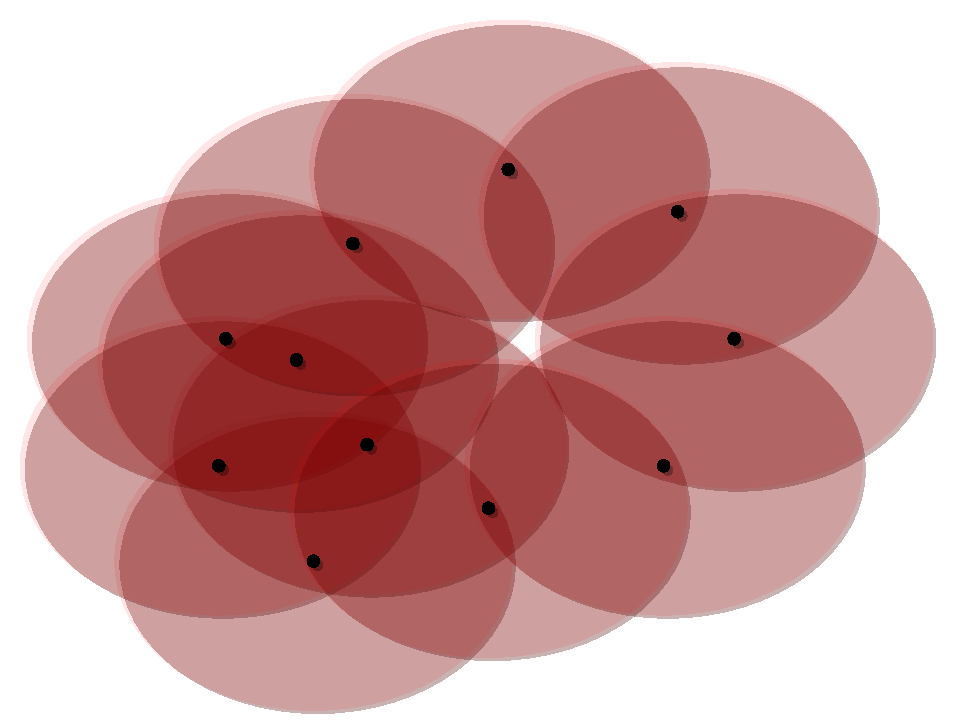
\includegraphics[scale=0.33]{figures/holes_cover.pdf}
    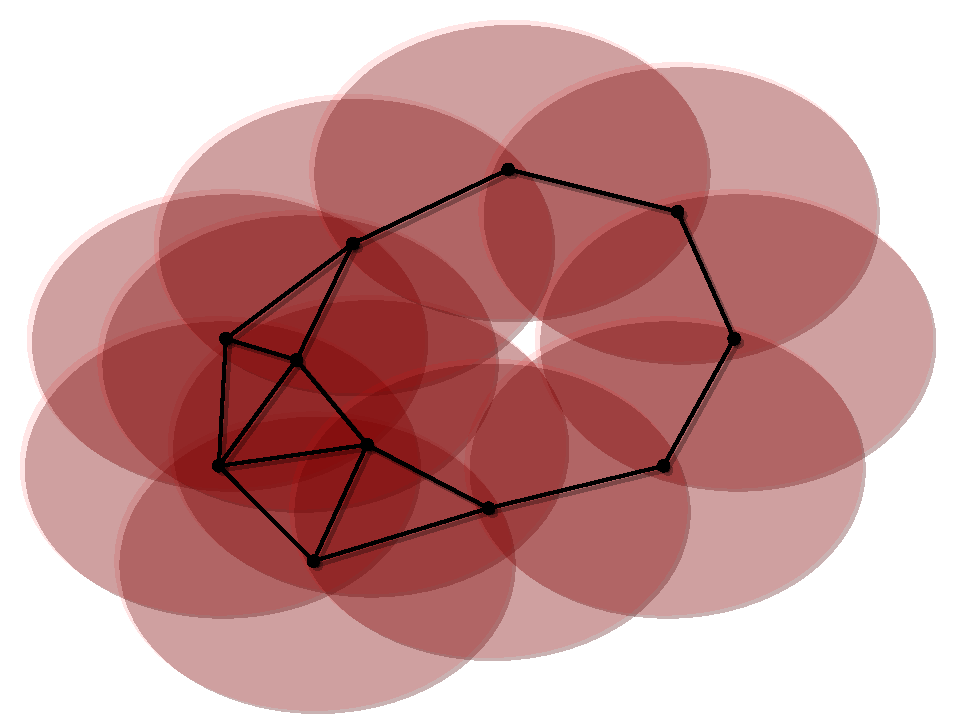
\includegraphics[scale=0.33]{figures/holes_edges.pdf}
    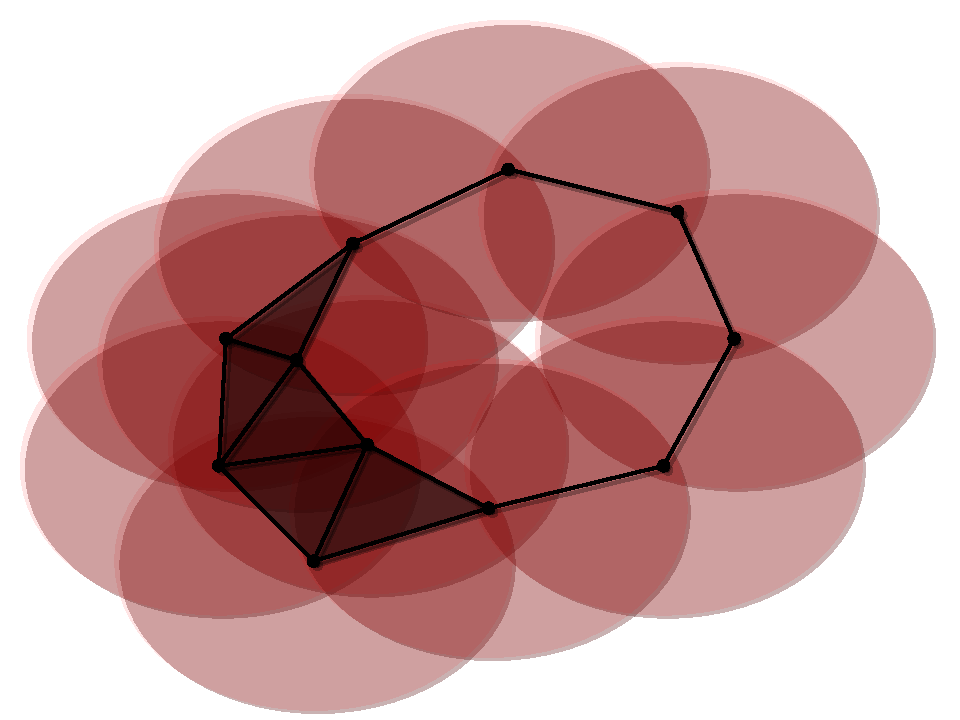
\includegraphics[scale=0.33]{figures/holes_complex.pdf}
     \caption{}
     \label{fig:holes}
 \end{figure}

It is natural to think of a $k$-dimensional simplicial complex as the generalization of an undirected graph consisting of vertices and edges, collections of at most 2 vertices, to collections of sets of at most $k-1$ vertices.
Just as we have defined a hole in our graph $G$ as a cycle that cannot be filled with triangles, we define a $k$-dimensinal hole in a simplicial complex as a $k$-cycle that cannot be filled with $(k+1)$-simplices.
In the next section we will formally define $k$-cycles and introduce simplicial homology as a tool for identifying when and which cycles cannot be filled.

% As such, simplicial complexes serve offer a more robust discrete representation of high dimensional domains.
Let $K$ be a simplicial complex with 0-simplices $\{v\}$ for all $p\in P$, 1-simpices $\{u, v\}\subset P$ for each edge in $E$, and 2-simplices $\{u,v,w\}\subset P$ whenever $\{\{\{u,v\},\{v,w\},\{u,w\}\}\subset E$.
This particular simplicial complex is known as the Vietoris-Rips complex.
\begin{definition}
    The \textbf{(Vietoris-)Rips complex} is defined for a set $P$ at scale $\e > 0$ as
    \[ \rips^\e(P) = \left\{\sigma \subseteq P\mid \forall p,q\in\sigma,\ \dist(p, q)\leq\e\right\}. \]
\end{definition}
% This construction generalizes to higher dimensions, allowing us to identify not only holes in planar graphs, ``holes'' in any dimension $k$ as $(k-1)$-cycles in high dimensional simplicial complexes.

 % \begin{figure}[htbp]
 % \centering
 %     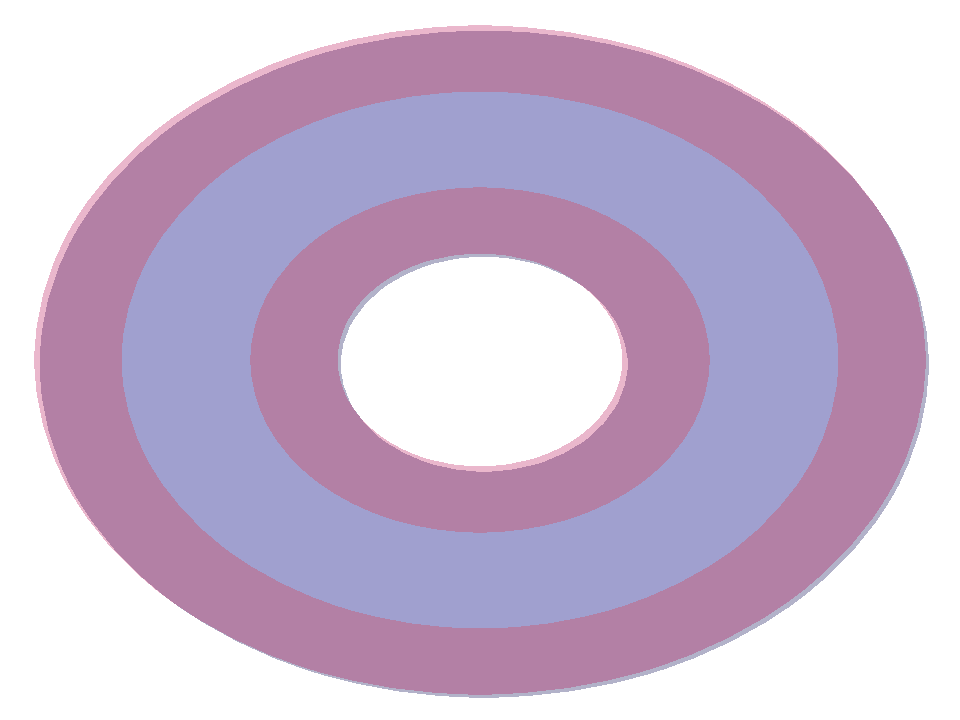
\includegraphics[scale=0.5]{figures/boundary_domain.pdf}
 %     % 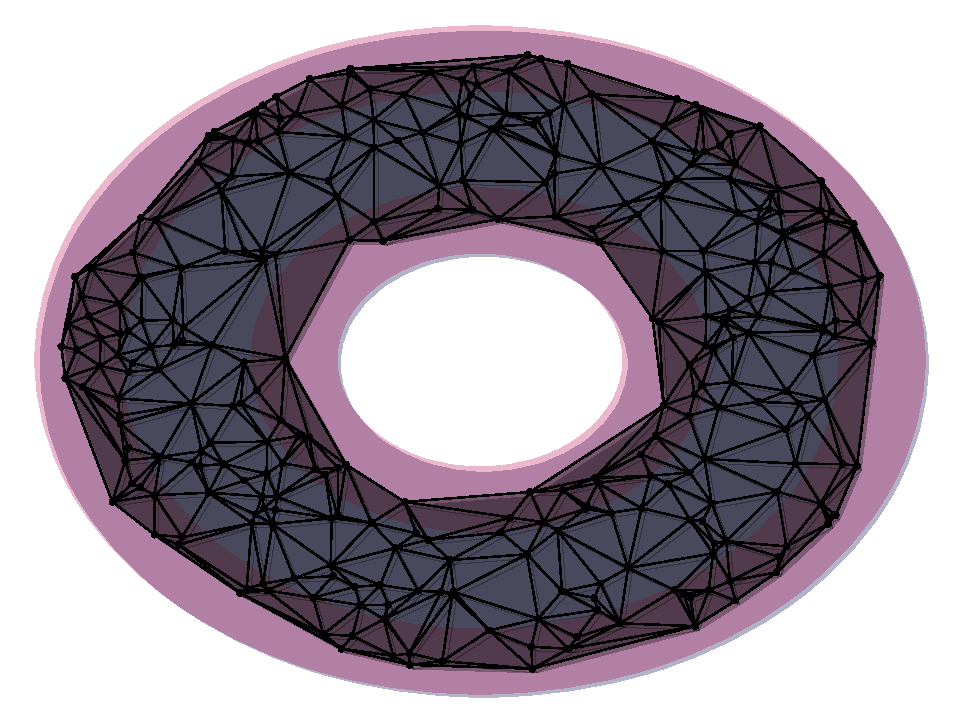
\includegraphics[scale=0.5]{figures/boundary_complex_domain.pdf}
 %     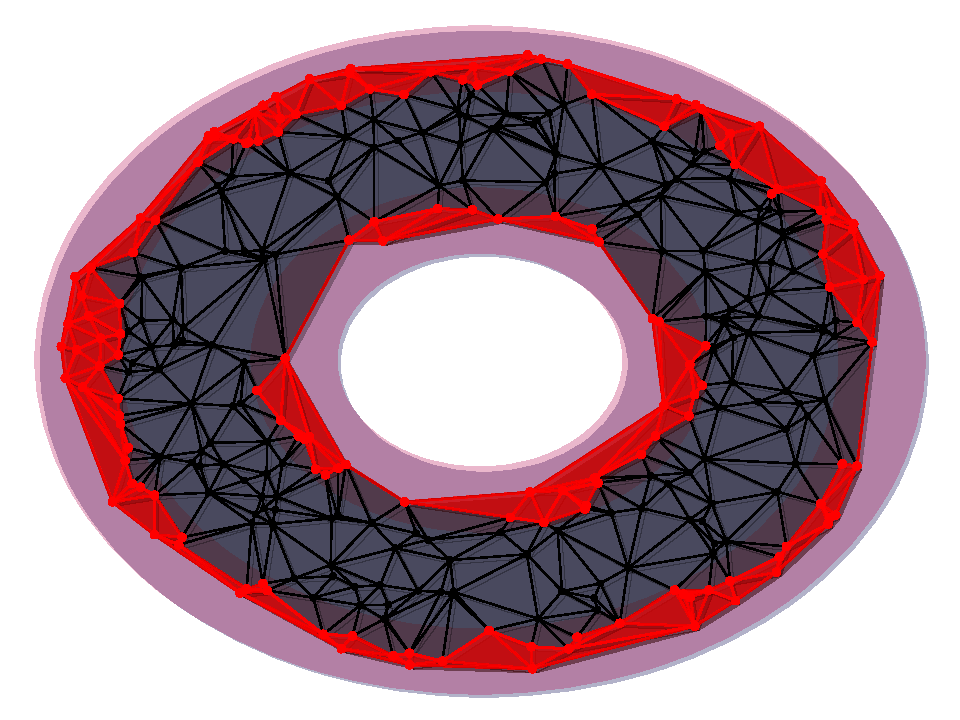
\includegraphics[scale=0.5]{figures/boundary_complex_domain_fence.pdf}
 %     % 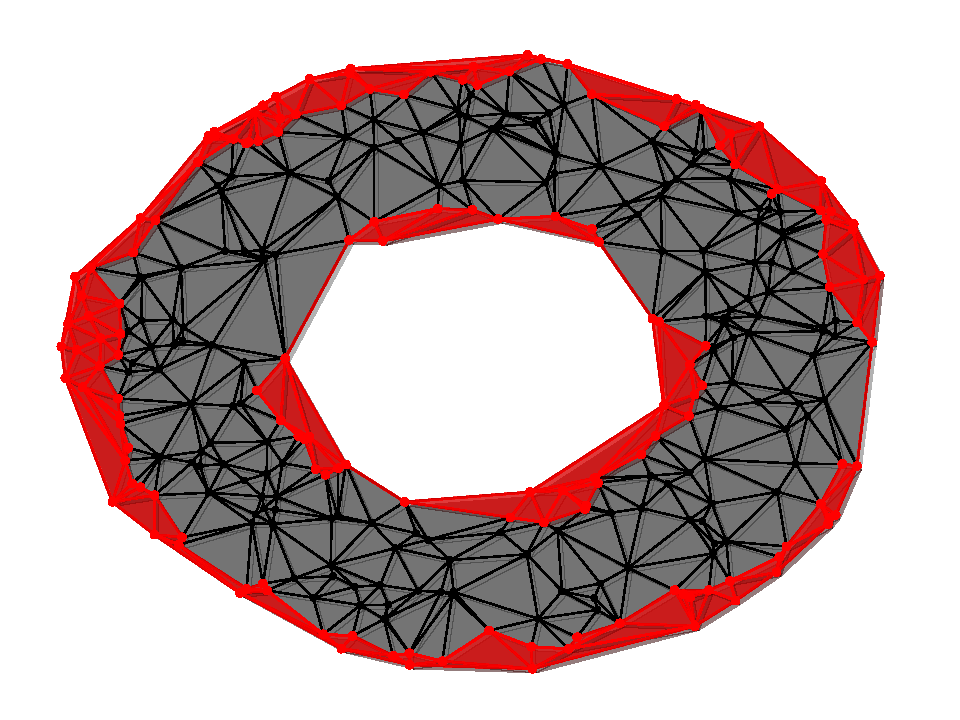
\includegraphics[scale=0.24]{figures/boundary_complex_fence.pdf}
 %      \caption{}
 %      \label{fig:boundary2}
 %  \end{figure}

\subsection{Coverage}

A subset $D$ of an domain $\D$ is covered by $P\subset$ at scale $\e > 0$ if every point $x\in D$ is within distance $\alpha$ at least one point in $P$.
\begin{definition}
    The \textbf{coverage region} of a point $p\in P$ at scale $\e > 0$ is defined
    \[\ball_\e(p) = \{x\in\D\mid \dist(x, p)\}.\]
\end{definition}
Let $P^\e$ to denote set of points in $\D$ within distance $\e$ of at least one point in $P$:
\[ P^\e = \bigcup_{p\in P}\ball_\e(p). \]
\begin{definition}
    Let $D, P\subset\D$.
    $D$ is \textbf{covered} by $P$ at scale $\e$ if $D\subseteq P^\e$.
\end{definition}
For this section we will assume that the coverage radius of our sensor network is equal to the radius of communication.
With this assumption we know that the converse problem is true: if a sensor network $P$ covers a domain at scale $\alpha$ the topology of the domain is reflected in $\rips^\alpha(P)$ however, as we will see this is in no way a tight bound on the minimal radius for coverage.

\begin{figure}[htbp]
\centering
    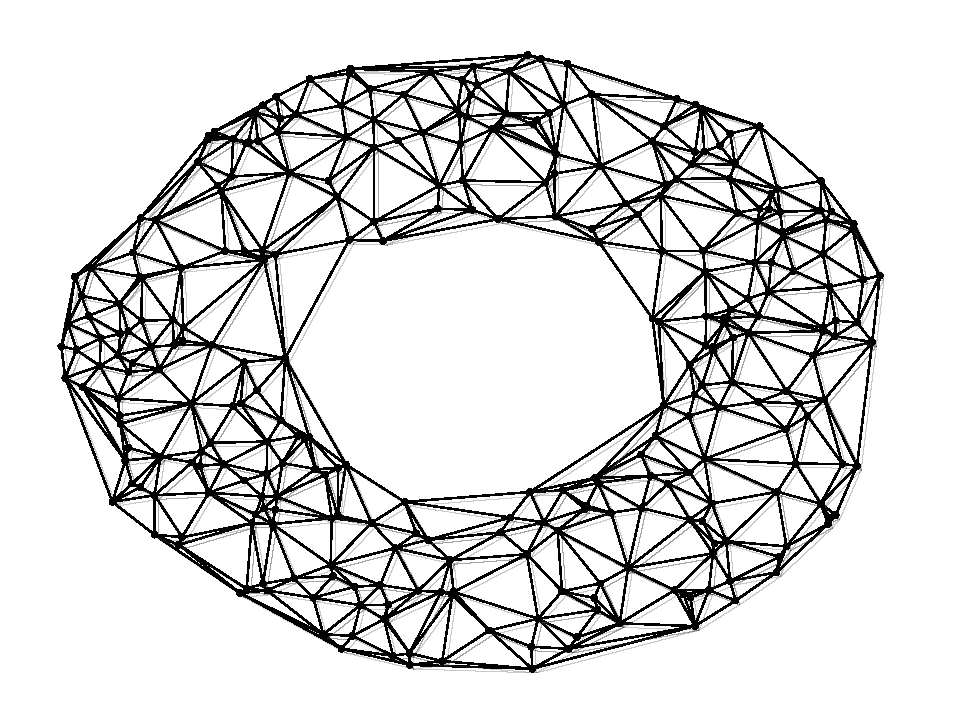
\includegraphics[scale=0.33]{figures/boundary_graph.pdf}
    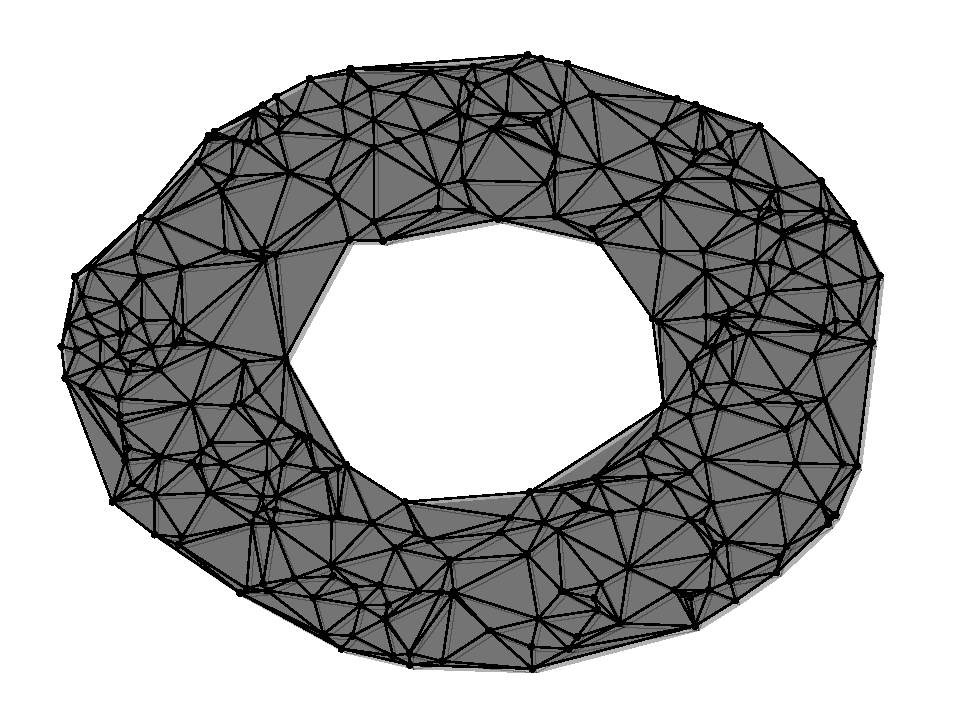
\includegraphics[scale=0.33]{figures/boundary_complex.pdf}
    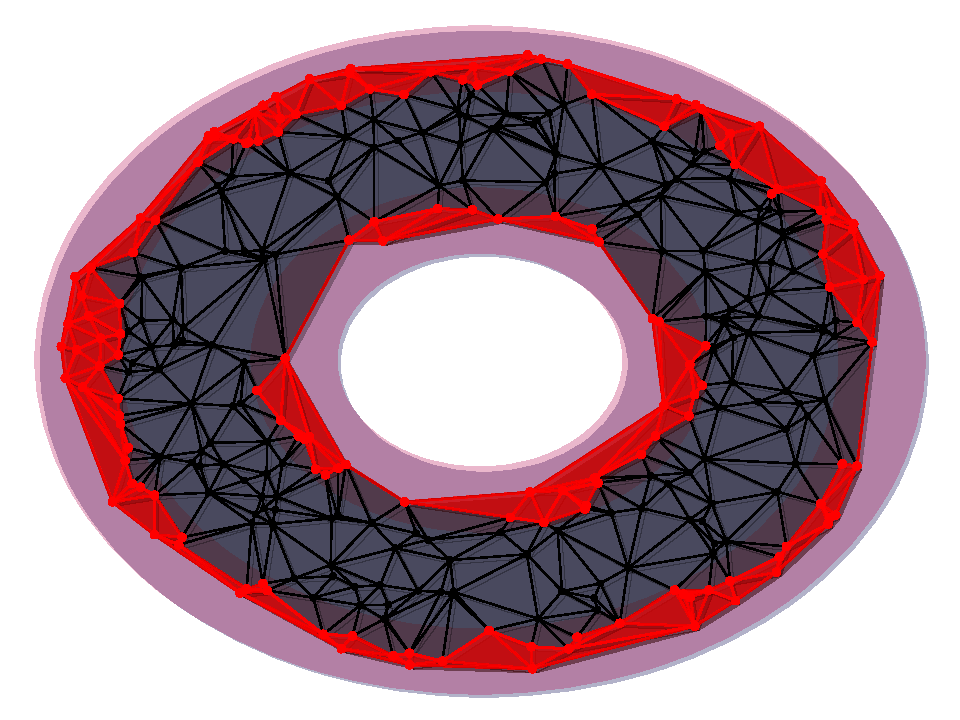
\includegraphics[scale=0.33]{figures/boundary_complex_domain_fence.pdf}
    % 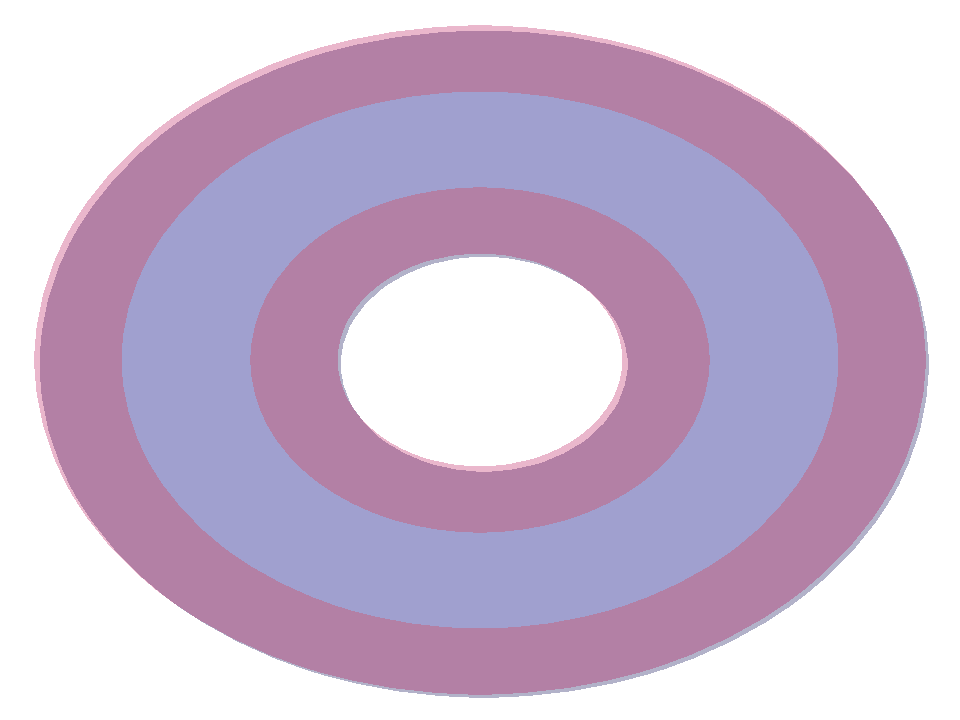
\includegraphics[scale=0.24]{figures/boundary_domain.pdf}
     \caption{}
     \label{fig:boundary1}
 \end{figure}

In order to \textit{verify} coverage by we need our network to sufficiently sample the extent of our domain.
Moreover, if there are gaps in coverage, are they due to insufficient sampling or a gap in the domain itself?
Let $\B\subset\D$ be the \textbf{boundary} of our domain and let our sensors detect whe the are within communication radius of $\B$.
Let $Q = \{p\in P\mid \min_{x\in\B}\dist(x, p)\}$ be the set of \textbf{boundary nodes} in $P$.
The set $Q$ induces a \textbf{subcomplex} $\rips^\alpha(Q)$ of $\rips^\alpha(K)$ restricted to nodes in $Q$.
% Assuming there are no holes in our network no path from a point in $P\setminus Q$ to a point outside our domain  without crossing a simplex in $K\mid_Q$.

\textbf{TODO} Section overview.
We will show how this construction is used to verify coverage of a specific subset of a bounded domain $\D$ with a tight bound on the coverage radius.

% Note that the communication radius is far from a tight bound on the coverage radius.

% section complexes (end)

% !TeX root = ../main.tex
\section{Homology} % (fold)
\label{sec:homology}

% Simplicial complexes not only provide a comprehensive discretization of continuous domains, but are the primary tool for concrete calculations in algebratic topology.
% In particular, the study of simplicial homology groups and its dual cohomology groups rely on simplicial complexes in order to study important topological invariants of a discretized space.
%
% \subsection{Homology}

The following vector spaces may be defined over any field $\F$, however we will assume the field $\F_2$ in order to avoid orienting the simplices in $K$.
Let $C_k(K)$ denote the vector space over some field $\F$ consisting of linear combinations of $k$-simplices in $K$, which form a basis for $C_k(K)$, known as \textbf{$k$-chains}.
These vector spaces are connected by \textbf{boundary maps} $\partial_k:C_k(K)\to C_{k-1}(K)$ which are linear transformations taking basis elements of $C_k(K)$ to the abstract sum of basis $(k-1)$-simplex faces.
The collection of chains and boundary maps forms a sequence of vector spaces known as the \textbf{chain complex} $\C = (C_*,\partial_*)$
\[
    \ldots\xrightarrow{\partial_{k+1}}
    C_k(K)\xrightarrow{\partial_{k}}
    C_{k-1}(K)\xrightarrow{\partial_{k-1}}
    \ldots\xrightarrow{\partial_2}
    C_1(K)\xrightarrow{\partial_{1}}
    C_0(K)\xrightarrow{\partial_0} 0.
\]

An important property of the boundary maps $\partial_k$ is that the composition of subsequent boundary maps is zero.
That is, for all $k$
\[
  \partial_k\circ\partial_{k-1} = 0.
\]
As a result the image of $\partial_{k+1}$, denoted $\im\partial_{k+1} = \{\partial_{k+1}c\mid c\in C_{k+1}(K)$ is a subspace of the kernel, $\ker\partial_k = \{c\in C_k(K)\mid \partial_k c = 0\}$, of $\partial_k$.
A \textbf{$k$-cycle} of $\C$ is a $k$-chain with empty boundary---an element of $\ker\partial_k$.
Two cycles in $\ker\partial_k$ are said to be \textbf{homologous} if they differ by an element of $\im\partial_{k+1}$.
This leads us to the definition of the \textbf{homology groups} of $K$ as quotient vector spaces $H_k(K)$ over $\F$, defined for $k\in\N$ as
\[
  H_k(K) := \ker\partial_k/\im\partial_{k+1}.
\]

The rank of a homology group is of particular importance and is known as the \textbf{Betti number} $\beta_k = \rank H_k(K)$.
These topological invariants can be thought of as counting the number of $k$-dimensional ``holes'' in a topological space, where $0$-dimensional holes are connected components, $1$-dimensional holes are loops, $2$-dimensional holes are voids, and so on.
Note that this is the same notion which motivated our use of simplicial complexes for determining coverage---a $1$-dimensional hole exists if a gap in a neighborhood graph cannot be filled by triangles.

\subsection{Relative Homology}

\begin{figure}[htbp]
\centering
    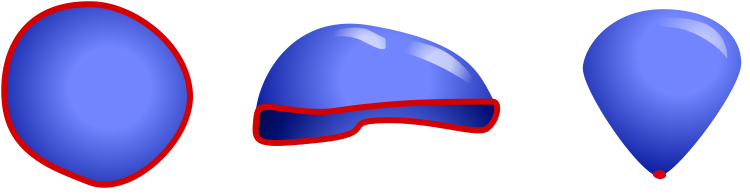
\includegraphics[scale=0.5]{figures/balloons1.png}\vspace{2ex}
    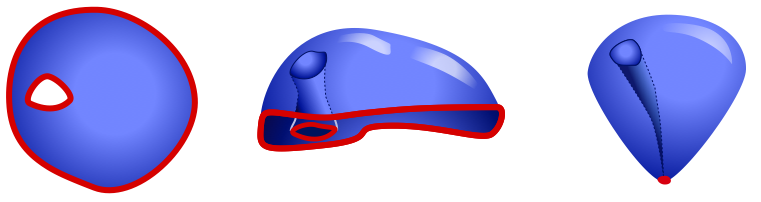
\includegraphics[scale=0.5]{figures/balloons3.png}
    \caption{(Left) Two connected, planar domains with boundaries (in red).
            We can gather some intuition for the relative homology of a pair $(\D,\B)$ by thinking about wrapping the interior of the domain around its boundary, and identifying all points in the boundary with a point (Right).
            Even with disconnected boundaries we know that $\beta_2 = \rank~ H_2(\D, \B) = 1$.  That is, there is just one enclosed void.}
    \label{fig:balloons1}
\end{figure}

For a simplicial complex $K$ let $L\subset K$ be a subcomplex of $K$.
Let $\C(K, L)$ denote the quotient chain complex of pairs $(C_k(K, L), \overline{\partial_k})$ where $C_k(K, L) = C_k(K)/C_k(L)$ consists of the chains on $K$ modulo chains on $L$, with the induced boundary maps $\overline{\partial_k}$ on the quotients.
Each relative chain is an equivalence class of chains in $K$ which are identical without the elements of $L$.
The \textbf{relative homology groups} $H_k(K, L)$ consists of homology classes of relative cycles - chains in $K$ whose boundaries vanish or lie in $L$.
That is, a relative cycle can either be a cycle in $K$ or a chain in $K$ with a boundary in $L$.

As we will see, relative homology provides a powerful representation of a bounded domain that is particularily suited to verifying coverage of a sensor network.
Let $\D$ be a bounded domain with boundary $\B\subset\D$.
For illustrative purposes assume $\D$ is a connected, compact subset of the euclidean plane $\R^2$ so that certain properties of the relative homology of the pair $(\D, \B)$ are known.
Namely, there is exactly one equivalence class in $H_2(\D, \B)$, as illustrated in Fig.~\ref{fig:balloons1}.
We can think of the quotient as an identification of points in the boundary, illustrated by wrapping the planar domain around a single point in $\R^3$.
As the domain is compact this creates a single void corresponding to the one generator in $H_2(\D, \B)$.

\begin{figure}[htbp]
\centering
    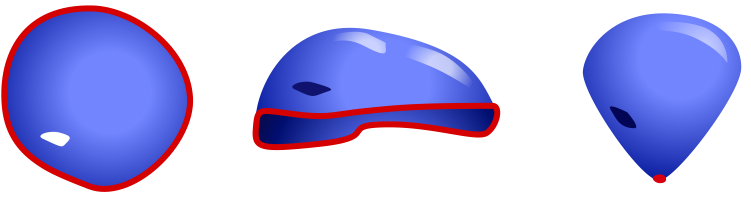
\includegraphics[scale=0.5]{figures/balloons2.png}
    \caption{If there is a gap in the domain that is not a part of the boundary then $\beta_2 = \rank~ H_2(\D, \B) = 0$ as there is no void.}
    \label{fig:balloons2}
\end{figure}

Now suppose our network $P$ covers the domain at some scale $\alpha > 0$ such that there are no gaps (1-cycles) in $\rips^\alpha(P)$.
The subset $Q = \{p\in P\mid \ball_\alpha(p)\cap\B\neq\emptyset\}$ of points within distance $\alpha$ of $\B$ induces a subcomplex $\rips^\alpha(Q)$ of $\rips^\alpha(K)$.
Under our assumptions, the relative homology $H_2(\rips^\alpha(K), \rips^\alpha(Q))$ should reflect that of the domain.
A gap in coverage can be thought of as ``popping the balloon'' in the sense that, if we wrap the simplices of $\rips^\alpha(K)$ around those in $\rips^\alpha(Q)$ we would have no void---the gap provides a hole through which the ``air'' can escape, as illustrated in Fig.~\ref{fig:balloons2}.

\subsection{Functions and Filtrations}

\begin{figure}[htbp]
\centering
    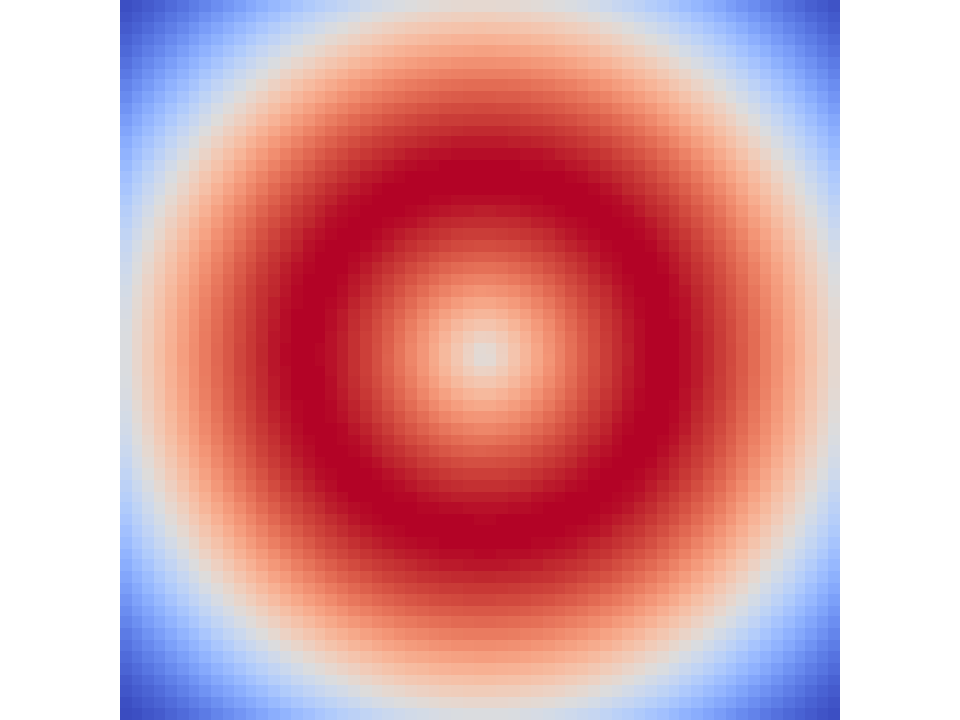
\includegraphics[scale=0.45]{figures/fgrid.pdf}
    % 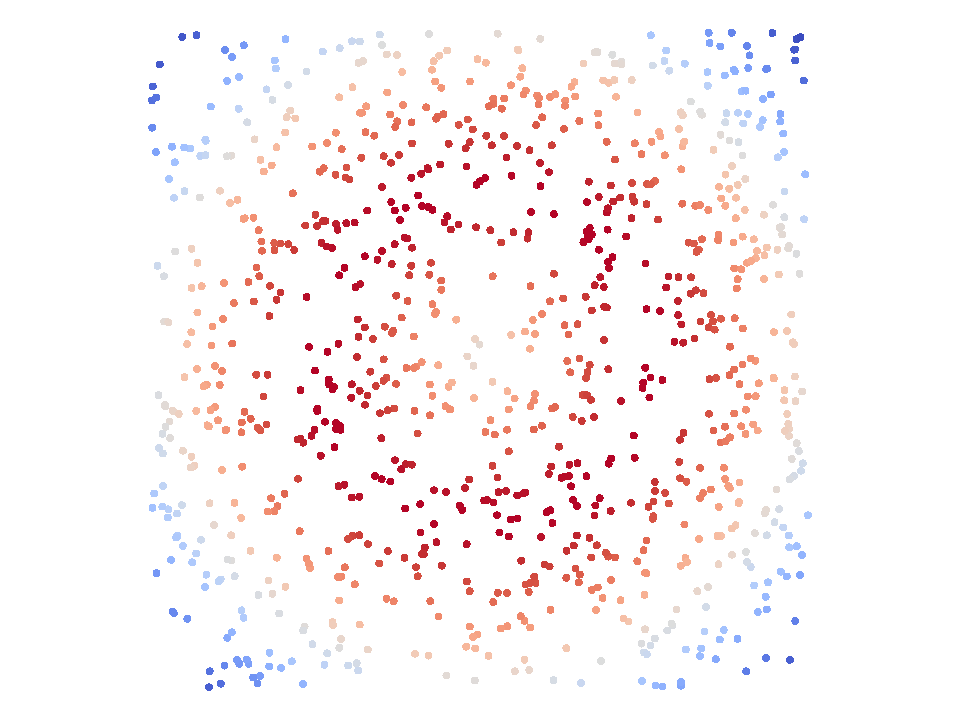
\includegraphics[scale=0.45]{figures/fsample.pdf}
    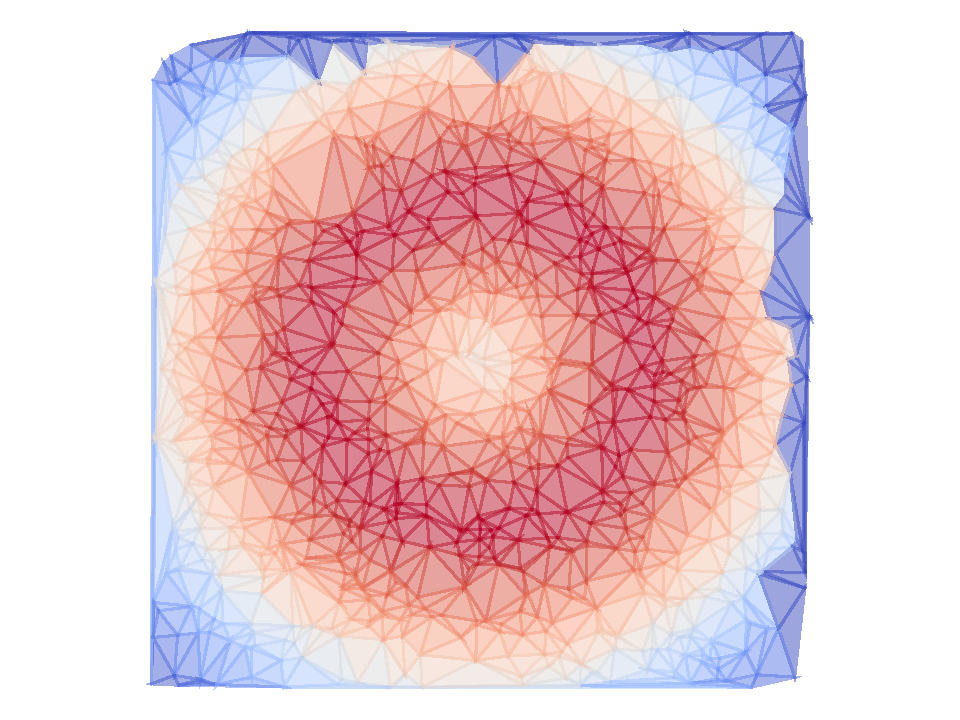
\includegraphics[scale=0.55]{figures/fcomplex.pdf}
    \caption{(Left) Continuous function on the plane.
            % (Middle) Function values on random sample.
            (Right) Function values on a random sample extended to a continuous piecewise linear approximation on a 2-dimension simplicial as the $z$-axis.}
    \label{fig:function}
\end{figure}

Suppose we have some real valued function $f:\D\to\R$ and endow our sensors with the ability to measure this function at their points $P$.
If we know our network covers the domain we may construct a simplicial complex which captures its topology in a discrete structure.
We may therefore integrate the sparse measurements provided by the sensors throughout the simplicial complex to capture the topology of the function itself.
Not only do we now have a discrete approximation of the function but an ordering on the simplices of the complex which may be used to explore the evolution of the topological structure of the function.

This leads to a more general notion defined for a sequence of topological spaces, which we may take as sublevel sets of the function on the domain.
\begin{definition}
    Let $f:\D\to\R$ be a function on a topological domain $\D$ and let $I_0, I_1,\ldots$ be a sequence of intervals $I_i = [a_i, b_i)$ that covers the image of $f$ on $\D$.
    Let and $X_i = \{x\in\D\mid a_i\leq f(x) < b_i\}$ be topological subspaces connected by inclusion maps $X_i\to X_{i+1}$.
    A \textbf{filtration} is the resulting sequence of topological spaces
    \[X_0\to X_1\to\ldots X_i\to X_{i+1}\to\ldots .\]
\end{definition}
A filtration $\{K_i\}_{i=1,\ldots,n}$ may also be interpreted as a sequence of simplicial maps, each an inclusion $K_i\to K_{i+1}$.
This induces an algebraic sequence of homomorphisms on homology by functoriality, for all $k$:
\[ H_k(X_0)\to H_k(X_1)\to\ldots\to H_k(X_i)\to H_k(X_{i+1})\to\ldots . \]
This sequence encodes the local topological changes that occur at each step of the filtration.
Global information is encoded in terms of the \textbf{birth} and \textbf{death} of homology classes, represented as a \textbf{persistence diagram} or \textbf{barcode}.

% \vspace{0.25in}
% \textbf{TODO} Persistence diagram of a function on a simplicial complex
% \vspace{0.25in}

\begin{figure}[htbp]
\centering
    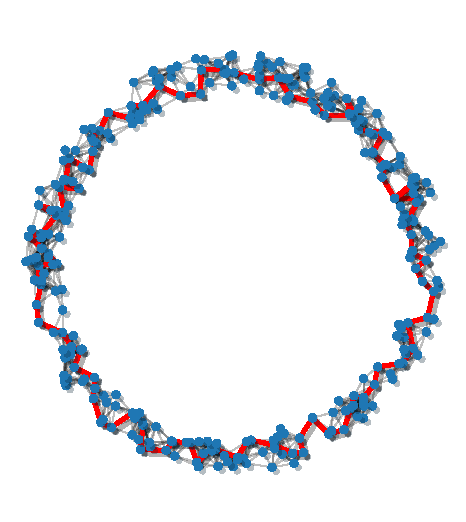
\includegraphics[scale=0.9]{figures/homology_cycle.pdf}\hspace{10ex}
    % 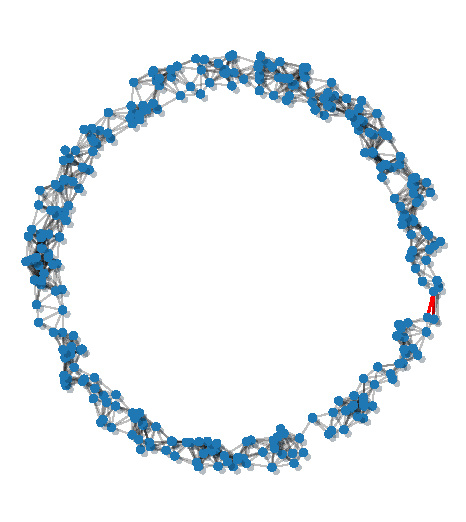
\includegraphics[scale=0.6]{figures/cohomology_cocycle.pdf}
    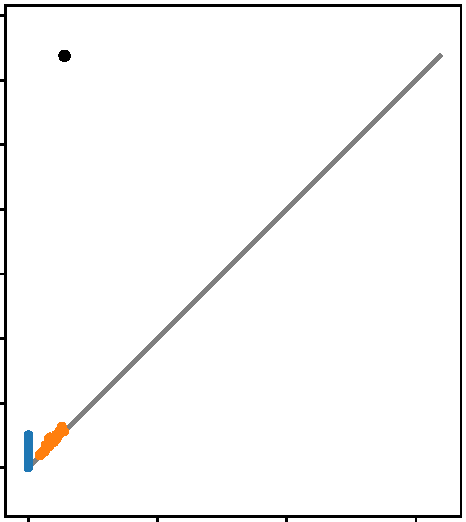
\includegraphics[scale=0.8]{figures/homology_dgm.pdf}
    \caption{The representative cycle of a significant feature in the persistent homology of rips filtration of a noisy circle.
            The birth of the feature indicated on the persistence diagram (right) corresponds to the scale of the rips complex shown (left) when the circle, a 1-cycle, is born.
            The death of this feature corresponds to the scale of the rips complex at a larger scale (not shown) when a triangle first fills the interior of the circle.
            This scale is approximately the length of the edges in the smallest equilateral triangle with sample points as vertices that contains the centroid of the sample.
            This illustrates the geometric information encoded in the persistence diagram of geometric complexes as it is within a constant factor of the radius of the circle.}
    \label{fig:cycle_diagrams}
\end{figure}

Given a simplicial complex $K$ on a set of points $P\subset\D$ and a function $f:\D\to\R$ we may construct a filtration $\{K_i\}_{i=1,2,\ldots}$ by ordering the simplices by their function values.
For example, $f(\sigma) = \max_{v\in\sigma} f(v)$ for any simplex $\sigma\in K$.
The resulting filtration is now a sequence of simplicial maps, each an inclusion $K_i\to K_{i+1}$, which induces a sequence of homology groups.

\subsection{Persistent Homology}

\begin{figure}[htbp]
\centering
    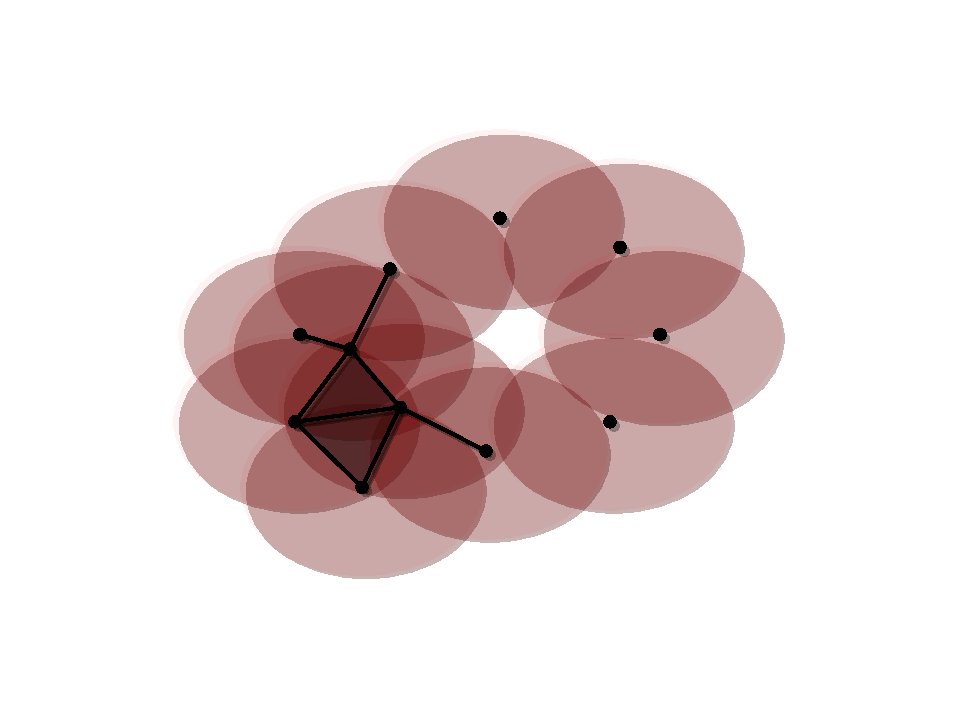
\includegraphics[scale=0.4]{figures/persist06.pdf}
    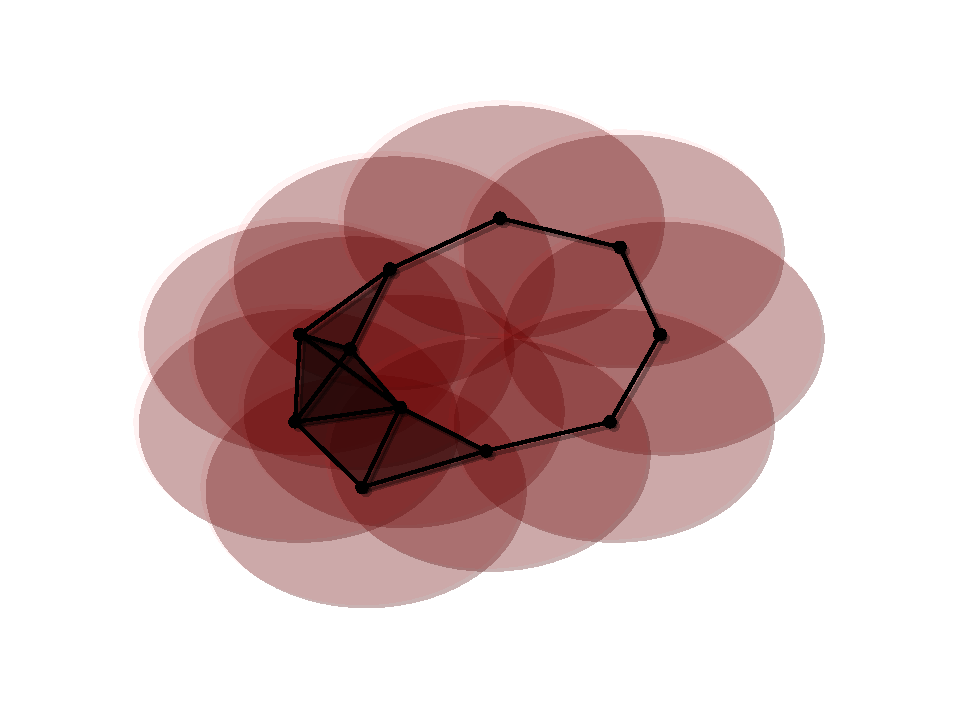
\includegraphics[scale=0.4]{figures/persist08.pdf}
    % 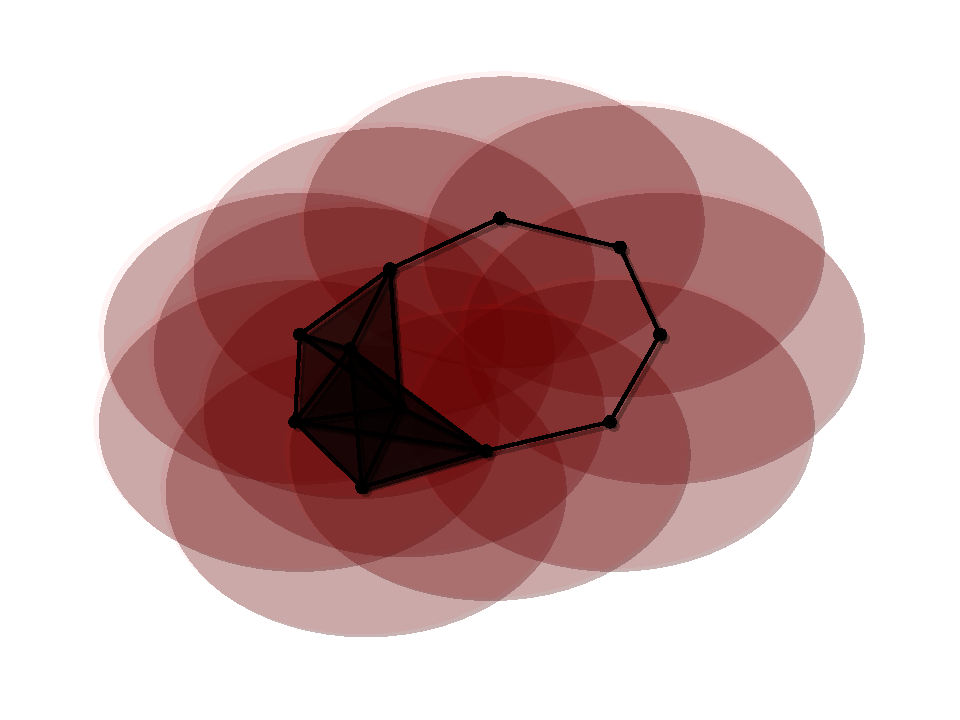
\includegraphics[scale=0.4]{figures/persist10.pdf}
    % 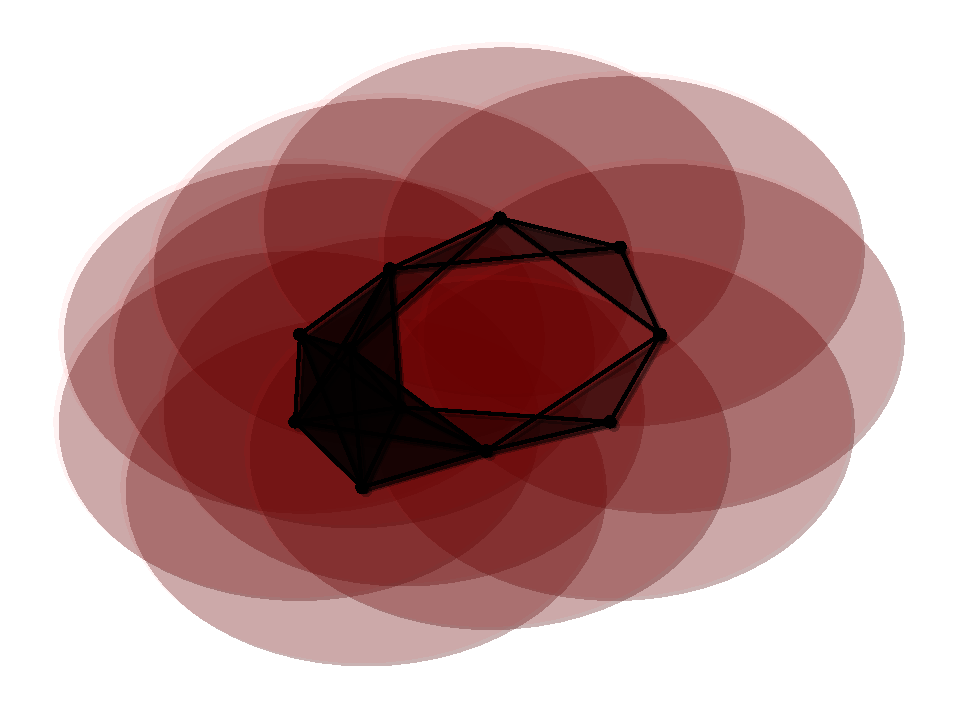
\includegraphics[scale=0.4]{figures/persist12.pdf}
    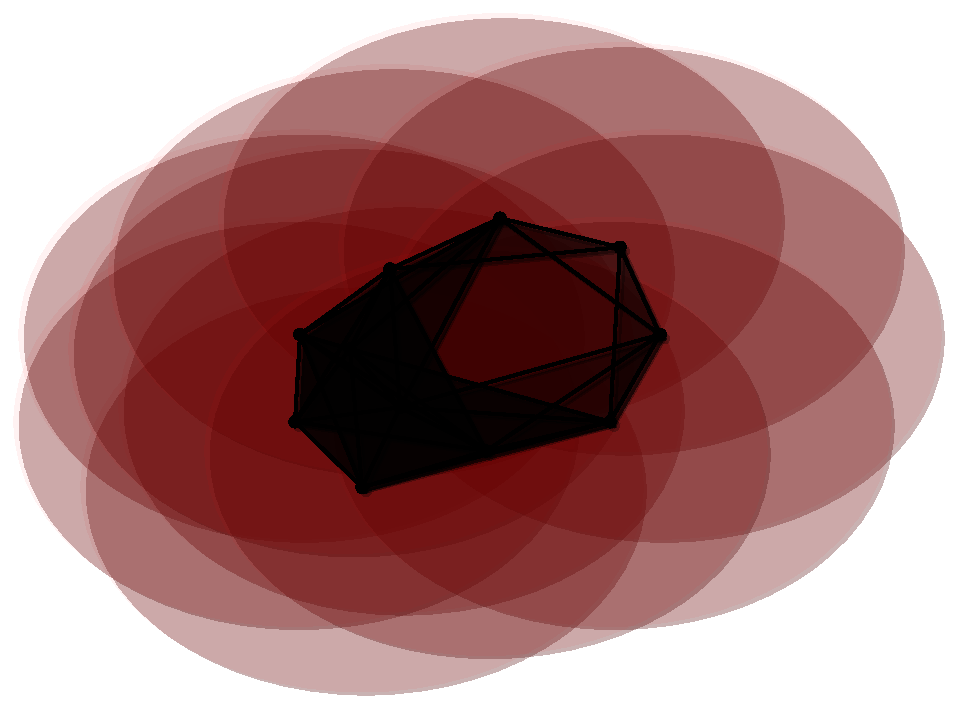
\includegraphics[scale=0.4]{figures/persist14.pdf}
    \caption{A filtration of rips complexes at scales 0.6, 0.8, and 1.4 illustrating a point $(0.8, 1.4)$ in the corresponding persistence diagram. The 1-cycle that is born at scale 0.8 persists until it dies at scale 1.4.}
    \label{fig:persist}
\end{figure}

% \vspace{0.25in}
% \textbf{TODO} ``Metric'' persistence.
% \vspace{0.25in}

% Topological data analysis is an emerging field in the intersection of data analysis and algebraic topology which extends the notion of homology and cohomology groups to a more analytical tool known as \textbf{topological persistence}.
% Where simplicial homology identifies invariants of a static simplicial complex persistent homology tracks the evolution of a sequence of nested simplicial complexes which provide a more detailed topological signature, in addition to relevant geometric information.

Just as we can construct a filtration from a function on a simplicial complex we can construct a filtration from the metric induced on our sample by the domain.
Let $P$ be a finite metric space with $m$ points and let $K = \rips^\alpha(P)$ be the Rips complex of $P$ at scale $\alpha$ consisting of $n$ simplices.
We can order the simplices $\sigma_1,\ldots,\sigma_n$ by the minimum pairwise distance between their vertices by first applying an arbitrary ordering on the vertices $v_1,\ldots,v_m$ and letting $\sigma_i = \{v_i\}$ for $i=1,\ldots,m$ so that $K_i = \{\sigma_1,\ldots, \sigma_m\}$.
We can then build a filtration $\K = \{K_i\}_{i=1,\ldots,n}$ so that $K_i = \rips^\e(P)$ where $\e = \max_{u,v\in\sigma_i}\dist(u,v)$ by adding one simplex at a time, breaking ties first by dimension, then by the ordering on their constituent vertices.
A $k$-dimensional feature is identified when a $(k+1)$-simplex $\sigma$ is added that kills a $k$-cycle $\gamma$.
In the persistence diagram, this feature would be represented by a point $(b, d)$ where $b$ is the smallest scale for which the $k$-cycle appears
\[ \tau\in\rips^b(P)\text{ for all }\tau\in\gamma\]
and $d = \max_{u,v\in\sigma}\dist(u,v)$ is the scale at which $\sigma$ enters the filtration.
The result is a collection of points $(b_i, d_i)$ in the plane for each dimension $k$ known as the persistence diagram, denoted $\dgm_k(\K)$.
A persistence diagram is depicted on the right in Fig.~\ref{fig:persist}.

% section homology (end)

% !TeX root = ../main.tex
\section{Cohomology} % (fold)
\label{sec:cohomology}

A \textbf{cochain complex} is a sequence $\tilde{\C} = (C^*, \delta_*)$ of $\R$-modules $C^k$ consisting of \textbf{cochains} and module homomorphisms known as \textbf{coboundary maps} $\delta_k:C^k\to C^{k+1}$.
As in homology we have the property that $\delta_{k+1}\circ\delta_k = 0$ for all $k$, leading to a familiar definition of the \textbf{cohomology} of $\tilde{\C}$
\[ H^k(\C) = \ker\delta_k/\im\delta_{k-1}.\]
The equivalence classes of $H^k(\C)$ consist of \textbf{$k$-cocycles}: elements of $\ker\delta_k$ that differ by a \textbf{$k$-coboundary} in $\im\partial_{k-1}$.
Such cocycles are said to be \textbf{cohomologous} if they belong to the same equivalence class in $H^k(\C)$.

The simplest construction of a cochain complex is to dualize a chain complex.
For a chain complex $(C_*,\partial_*)$ define $C^k$ to be the module of homomorphisms $\psi:C_k\to\R$.
The coboundary maps $\delta_k$ are defined for cochains $\psi:C_k\to\R$ and $k$-simplices $\sigma\in K$ as
\[\delta_k\psi(\sigma) = \psi(\partial_k\sigma).\]
It is in this sense that the cohomology $H^k(\tilde{\C})$ of a cochain complex $\tilde{\C}$ constructed from a chain complex $\C$ is the algebraic dual of the homology $H_k(\C)$ of $\C$.
Moreover, the \textbf{Universal Coefficient Theorem} implies that, for finite dimensional homology groups, there is an isomorphism between homology and cohomology groups.
It follows that there is an isomorphism between the persistent homology and \textbf{persistent cohomology} of a filtration $\K$.

While simplicial homology identifies equivalence classes of cycles in a chain complex simplicial cohomology instead identifies equivalence classes of homomorphisms from the chain complex to a field.
In essence, homology and cohomology offer different perspectives that reveal the same structure, homology rooted in geometry and cohomology in algebra.
As we will see the language of cohomology offers a more robust setting for using the algebraic structure of cocycles.

\subsection{Representative Cycles and Cocycles}

Let $K = \rips^\alpha(P)$ be the rips complex of a finite metric space $P$.
We can find a basis for each homology group $H_p(K)$ and cohomology group $H^p(K)$ consisting of $p$-cycles and $p$-cocycles, respectively.
In general, $p$-cycles represent $p$-dimensional holes in the simplicial complex $K$, where $p$-cocycles can be understood as ``blocking chains.''

\begin{figure}[htbp]
\centering
    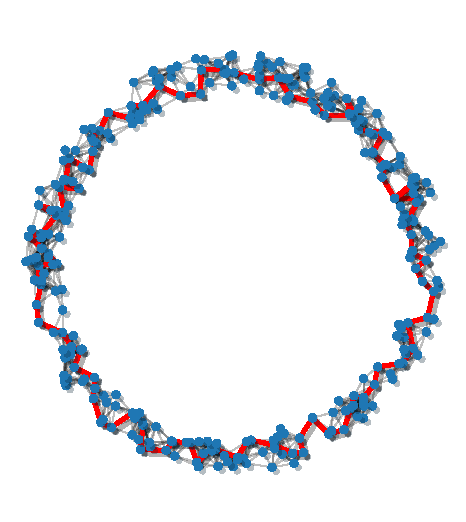
\includegraphics[scale=1.]{figures/homology_cycle.pdf}
    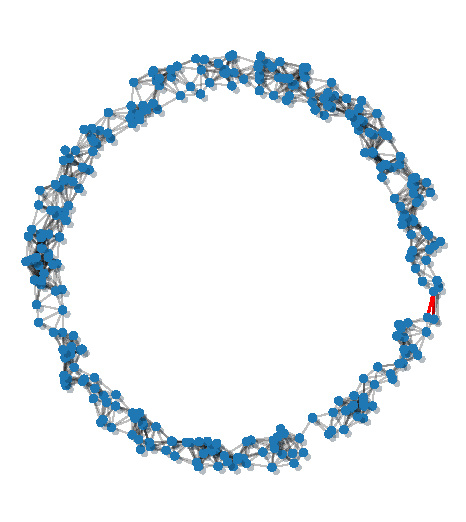
\includegraphics[scale=1.]{figures/cohomology_cocycle.pdf}
    % 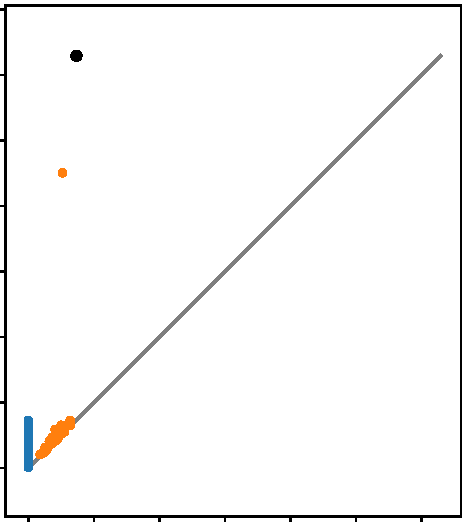
\includegraphics[scale=0.66]{figures/circular_dgm1.pdf}
    \caption{Consider a noisy sample $X$ of the 1-sphere, or circle, $\mathbb{S}^1$ with radius 1.
            Let $K = \rips^\e(X)$ for $\e\approx 0.14$, 1-skeleton shown.
            (Left) In red, the edges of a representative cycle of $H_1(K)$.
            (Right) In red, the edges of a representative cocycle of $H^1(K)$.
            Note that while the representative cycle clearly identifies equivalence class of 1-cycles of $X$, all paths around the circle, the representative cocycle represents the class of ``blocking'' cochains.}
    \label{fig:cycles}
\end{figure}

\subsection{Circular Coordinates}

Cocycles are particularily useful in distributing the information contained in each cohomology basis element throughout a simplicial complex.
This is one application of the theory of discrete exterior calculus, which we will illustrate with an algorithm presented by de Silva et al.~\cite{desilva09persistent}.
The work uses representative cocycles of features in persistent cohomology to construct a circle-valued function on the vertex set referred to as \textbf{circular coordinates}.
The distinction is made with Cartesian coordinates which are often viewed as values on a line (an axis).

\begin{figure}[htbp]
\centering
  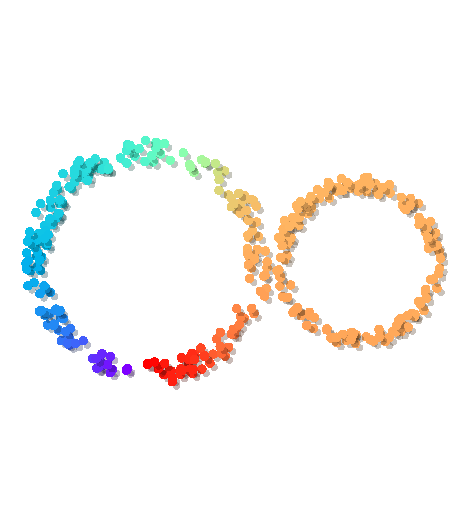
\includegraphics[scale=0.8]{figures/circular_coords1.pdf}
  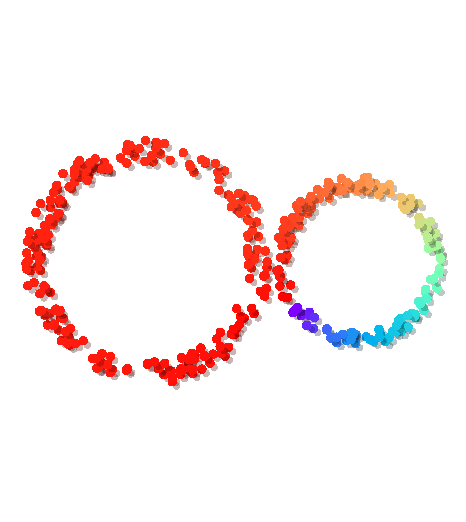
\includegraphics[scale=0.8]{figures/circular_coords2.pdf}\\\vspace{-7ex}
  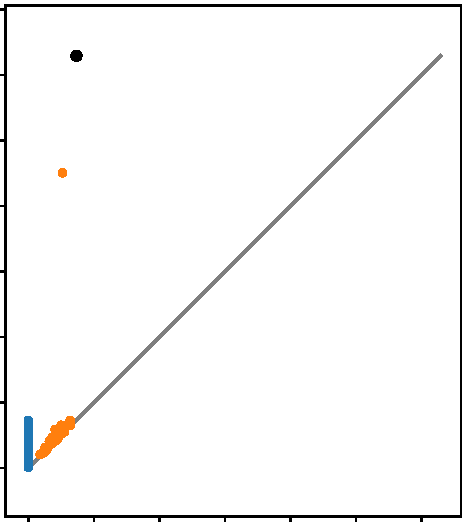
\includegraphics[scale=0.5]{figures/circular_dgm1.pdf}\hspace{1.3in}
  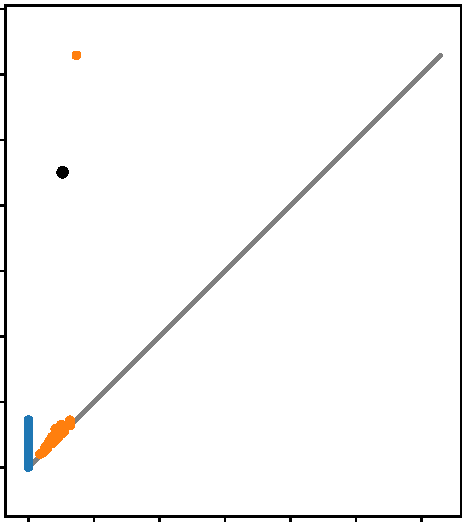
\includegraphics[scale=0.5]{figures/circular_dgm2.pdf}
   \caption{(Top) Circular coordinates as colorings on a set of points $P$ sampled from two noisy circles with radii 1 and 0.7.
        The two coordinates were constructed from representative 1-cocycles corresponding to persistent features in the persistent cohomology of the rips complex of $P$ (bottom).
        Note that each representative cocycle yeilds coordinates that are localized to the corresponding feature.}
   \label{fig:circular}
\end{figure}

Let $K$ be a simplicial complex constructed over a point cloud $P$ at some scale $\e_{max}$.
The algorithm first computes the persistent cohomology of $K$ over a prime field $\F_p$ for prime $p > 2$.
Any point $(b, d)$ in the 1-dimensional persistence diagram corresponds to a representative cocycle $\alpha_p\in C^1(K;\F_p)$.
Let $K^\e$ be the subcomplex of $K$ for some $\e\leq \e_{max}$ in the interval $[b, d]$ and $\alpha^\e_p\in C^1(K^\e;\F_p)$ be the restriction of $\alpha_p$ to simplices in $K^\e$.
For our calculations we chose the midpoint $\e = \frac{b+d}{2}$.
Moving forward let $K = K^\e$ and $\alpha_p = \alpha^\e_p$.

Next, ``lift'' the cocycle $\alpha_p$ over a prime field to an integer cocycle $\alpha\in C^1(K;\Z)$ which reduces to $\alpha_p$ modulo $p$.
In practice we can almost always construct $\alpha$ by taking the coefficients of $\alpha_p$ in $\F_p$ and replacing them with integers in the correct congruence class modulo $p$, preferring coefficients close to zero in the range
\[ \{-(p-1)/2,\ldots,-1,0,1,\ldots,(p-1)/2\}. \]
There are some edge cases in which the boundary $\delta_1\alpha\neq 0$, in which case $\alpha$ is not a valid integer cocycle, however for the sake of brevity we will assume that $\delta_1\alpha = 0$.

Noting that any integer cocycle $\alpha\in C^1(K;\Z)$ is also a real cocycle in $C^1(K;\R)$ we would now like to find the ``smoothest'' real cocycle $\overline{\alpha}\in C^1(K;\R)$ that is cohomologous to $\alpha$.
Such a cocycle is known as a \textbf{harmonic cocycle} representing the cohomology class $[\alpha]$.
Each of the spaces $C^i(X;\R)$ comes with a natural Euclidean metric: for $f\in C^0(K;\R)$, $\alpha\in C^1(K;\R)$ %, and $A\in C^2(K;\R)$
\begin{align*}
    \|f\|^2 = \sum_{p\in K^0} |f(p)|^2\\
    \|\alpha\|^2 = \sum_{e\in K^1} |\alpha(e)|^2 % \\
    % \|A\|^2 = \sum_{t\in K^2} |A(t)|^2
\end{align*}
where $K^k$ denotes the collection of $k$-simplices in $K$.
A circle-valued function $\theta$ is said to be ``smooth'' if its total variation across the edges of $K$ is small.
The variation of $\overline{\alpha}$ across edges $e\in K^1$ is captured by the terms $|\overline{\alpha}(e)|^2$, so we seek to minimize $\|\overline{\alpha}\|^2$.

\begin{proposition}
    Let $\alpha\in C^1(K; \R)$.
    There is a unique solution $\overline{\alpha}$ to the least-squares minimization problem
    \[ \argmin_{\overline{\alpha}} \{\|\overline{\alpha}\|^2\mid \exists f\in C^0(K;\R),\ \overline{\alpha} = \alpha + \delta_0 f\}.\]
    Moreover, $\overline{\alpha}$ is characterized by the equation $\delta_0^*\overline{\alpha} = 0$, where $\delta_0^*$ is the adjoint of $\delta_0$ with respect to the inner products on $C^0, C^1$.
\end{proposition}

We can integrate the resulting harmonic cocycle $\overline{\alpha}$ to obtain a circle-valued function $\theta$ on the vertex set $X^0$ as follows.
If $K$ is connected (if not, each connected component can be treated separately) select a starting vertex $x_0$ and set $\theta(x_0) = 0$.
Then find the shortest path from $x_0$ to each remaining vertex - when a new vertex $b$ enters the structure via an edge $e$ from vertex $a$ to $b$ assign $\theta(b) = \theta(a) + \overline{\alpha}(e)$.

% \vspace{0.25in}
% \textbf{TODO} Cochains as functions on simplicial complexes
% \vspace{0.25in}

% \subsection{Discrete Exterior Calculus}

 % and $\K = \{K_i\}_{i=1,\ldots,n}$ be a filtration of simplicial complexes $K_i = \rips^\alpha_i(P)$ for $\alpha_1 < \alpha_2 <\ldots < \alpha_{n-1} < \alpha_n = \alpha$.
 % While this does not have an immediate application to our investigation of coverage in homological sensor network it is a powerful tool which may be used for future research in coordinate free sensor networks.

% section cohomology (end)

% !TeX root = ../main.tex
\section{Homological Sensor Networks and the TCC} % (fold)
\label{sec:tcc}

Throughout we have been using the Rips complex as a discrete representation of our coverage domain by assuming our sensor's coverage radius is equal to their communication radius.
In fact, if the Rips complex of a sensor network at scale $\alpha$ has no gaps the minimum coverage radius required is a constant factor smaller than $\alpha$.
This Point is made clear by an interleaving of the Rips with another simplicial complex known as the \v Cech complex.

\begin{definition}
    The \textbf{\v Cech complex} of a finite collection of points $P$ at scale $\e > 0$ is defined
    \[ \cech^\e(P) := \left\{\sigma \subseteq P\mid \bigcap_{p\in \sigma}\ball_\e(p)\neq \emptyset \right\}. \]
\end{definition}
The \v Cech complex is a special case of a more general construction known as a the \textbf{nerve} $\N(\U)$ of a collection of sets $\U = \{U_i\}_{i\in I}$, where $I$ is any indexing set.
The nerve of $\U$ is defined as the simplicial complex with vertex set $I$ such that $\sigma\subseteq I$ is a simplex if and only if \[\bigcap_{i\in \sigma} U_i\neq \emptyset.\]
The collection $\U$ is a \textbf{good cover} if for each $\sigma\subset I$ the set $\bigcap_{i\in\sigma} U_i$ is contractible if it is nonempty.
The \textbf{nerve lemma} states that if $\U$ is a good cover then its nerve $\N(\U)$ is homotopy equivalent to $\bigcup_{i\in I} U_i$.
That is, for a set of nodes $P\subset\D$ such that $\U = \{\ball_\e(p)\mid p\in P\}$ is a good cover the nerve $\N(\U)$ is homotopy equivalent to $P^\e = \bigcup_{p\in P} \ball_\e(p)$.
It follows that the \v Cech complex $\cech_\e(P)$ of $P$ at scale $\e$ is a suitable representation of the coverage region $P^\e$.

In order to construct the \v Cech complex our sensors must be able to measure not only the proximity of neighboring nodes, but the precise distance between them.
Fortunately, the \v Cech and Rips complexes of a finite metric space are closely related by a result that follows from Jung's Theorem~\cite{jung01uber} relating the diameter of a point set $P$ and the radius of the minimum enclosing ball:
\begin{equation}\label{eq:jung_inclusion}
  \cech^\e(P)\subseteq\rips^\e(P)\subseteq\cech^{\jungd \e}(P)\subseteq\rips^{\jungd\e}(P),
\end{equation}
where the constant $\jungd = \sqrt{\frac{2d}{d+1}}$ (see~\cite{buchet15efficient}).

Equipped with this interleaving we are now ready to define all conditions necessary for verifying coverage in a coordinate-free sensor network.
Specifically, we will introduce a second radius of communication $\beta\geq 3\alpha$ that will allow us to lower $\alpha$, which will remain our coverage radius, so that homomorphism on (relative) homology induced by the inclusion of rips complexes $\rips^\alpha(P)\to\rips^\beta(P)$ reflects that of the \v Cech, and therefore the coverage domain.

\subsection{The Topological Coverage Criterion}

To recap, we have an unknown, bounded domain $\D$ with boundary $\B$ and a finite collection of sample points $P\subset\D$.
Each sensor, represented by a single point $p\in P$, can do the following:

\vspace{3ex}
\begin{center}
\setlength{\fboxsep}{2ex}
\fbox{\parbox{0.85\textwidth}{
    \begin{itemize}
        \item[a.]\textbf{(Communication Radii)} detect the presence, but not location or distance, of sensors within distances $\alpha > 0$ and $\beta \geq 3\alpha$, and discriminate between sensors within each scale,
        \item[b.]\textbf{(Coverage Radius)} cover a radially symmetric subset of the domain with radius $\alpha$,
        \item[c.]\textbf{(Boundary Detection)} detect the presence of the boundary $\B$ within distance $\alpha$.
    \end{itemize}
}}\end{center}\vspace{3ex}

\begin{definition}
    For a pair of sets $(\D, \B)$ such that $\B\subseteq \D$, we say that $\B$ \emph{surrounds} $\D$ if there is no path from $\D\setminus\B$ to $\comp{\D}$ that does not intersect $\B$.
    Formally, $\B$ surrounds $\D$ if and only if $H_0(\D\setminus \B) \cong H_0(\comp{\B}, \comp{\D})$, where $\comp{\D}$ denotes the complement of $\D$ in the ambient space containing $\D$.
\end{definition}

If such a pair satisfies the following conditions for $0 < 3\alpha\leq \beta$, we want to certify that a finite sample $P\subset\D$ covers $\D$ at scale $\alpha$ in the sense that $\D\setminus\B^{2\alpha}\subset P^\alpha$.
\euclidean{Although the TCC holds for more general spaces with a few technical assumptions (see~\cite{cavanna17when}) we will assume that our domain $\D$ is a subset of $\R^d$ for the sake of simplicity.}

\vspace{2ex}
\begin{center}
\setlength{\fboxsep}{2ex}
\fbox{\parbox{0.75\textwidth}{
% \vspace{1ex}\hspace{1ex}
\textbf{Geometric Assumptions}
    \begin{enumerate}
    \setcounter{enumi}{-1}
        \item \textbf{(The Domain)} \noeuclidean{$\D$ is a bounded, compact length space homeomorphic to a subset of $\R^d$}\euclidean{$\D$ is a bounded, compact subset of $\R^d$} and $\B\subseteq \D$ is closed and surrounds $\D$.
        \item \textbf{(Components are not too small)} $\hom_0(\D\setminus\B^{\alpha+\beta}\hookrightarrow \D\setminus\B^{2\alpha})$ is surjective.
        \item \textbf{(Components are not too close)} $\hom_0(\D\setminus\B^{2\alpha}\hookrightarrow (\D\setminus \B)^{2\alpha})$ is injective.
    \end{enumerate}
}}\end{center}\vspace{4ex}

% Lemma~\ref{lem:shrunken_to_relative} allows us talk about the homology of a subset of the domain $\D\setminus\B^\e$ in terms of relative homology.
% \begin{lemma}\label{lem:shrunken_to_relative}
%     If $\B$ surrounds $\D$, then for all $\e>0$, $\hom_0((\D\setminus\B^{\e},\emptyset)\hookrightarrow (\comp{\B^{\e}},\comp{\D^{\e}}))$ is an isomorphism.
% \end{lemma}

\begin{wrapfigure}{r}{0.5\linewidth}%
    \centering
    \vspace{-5ex}
    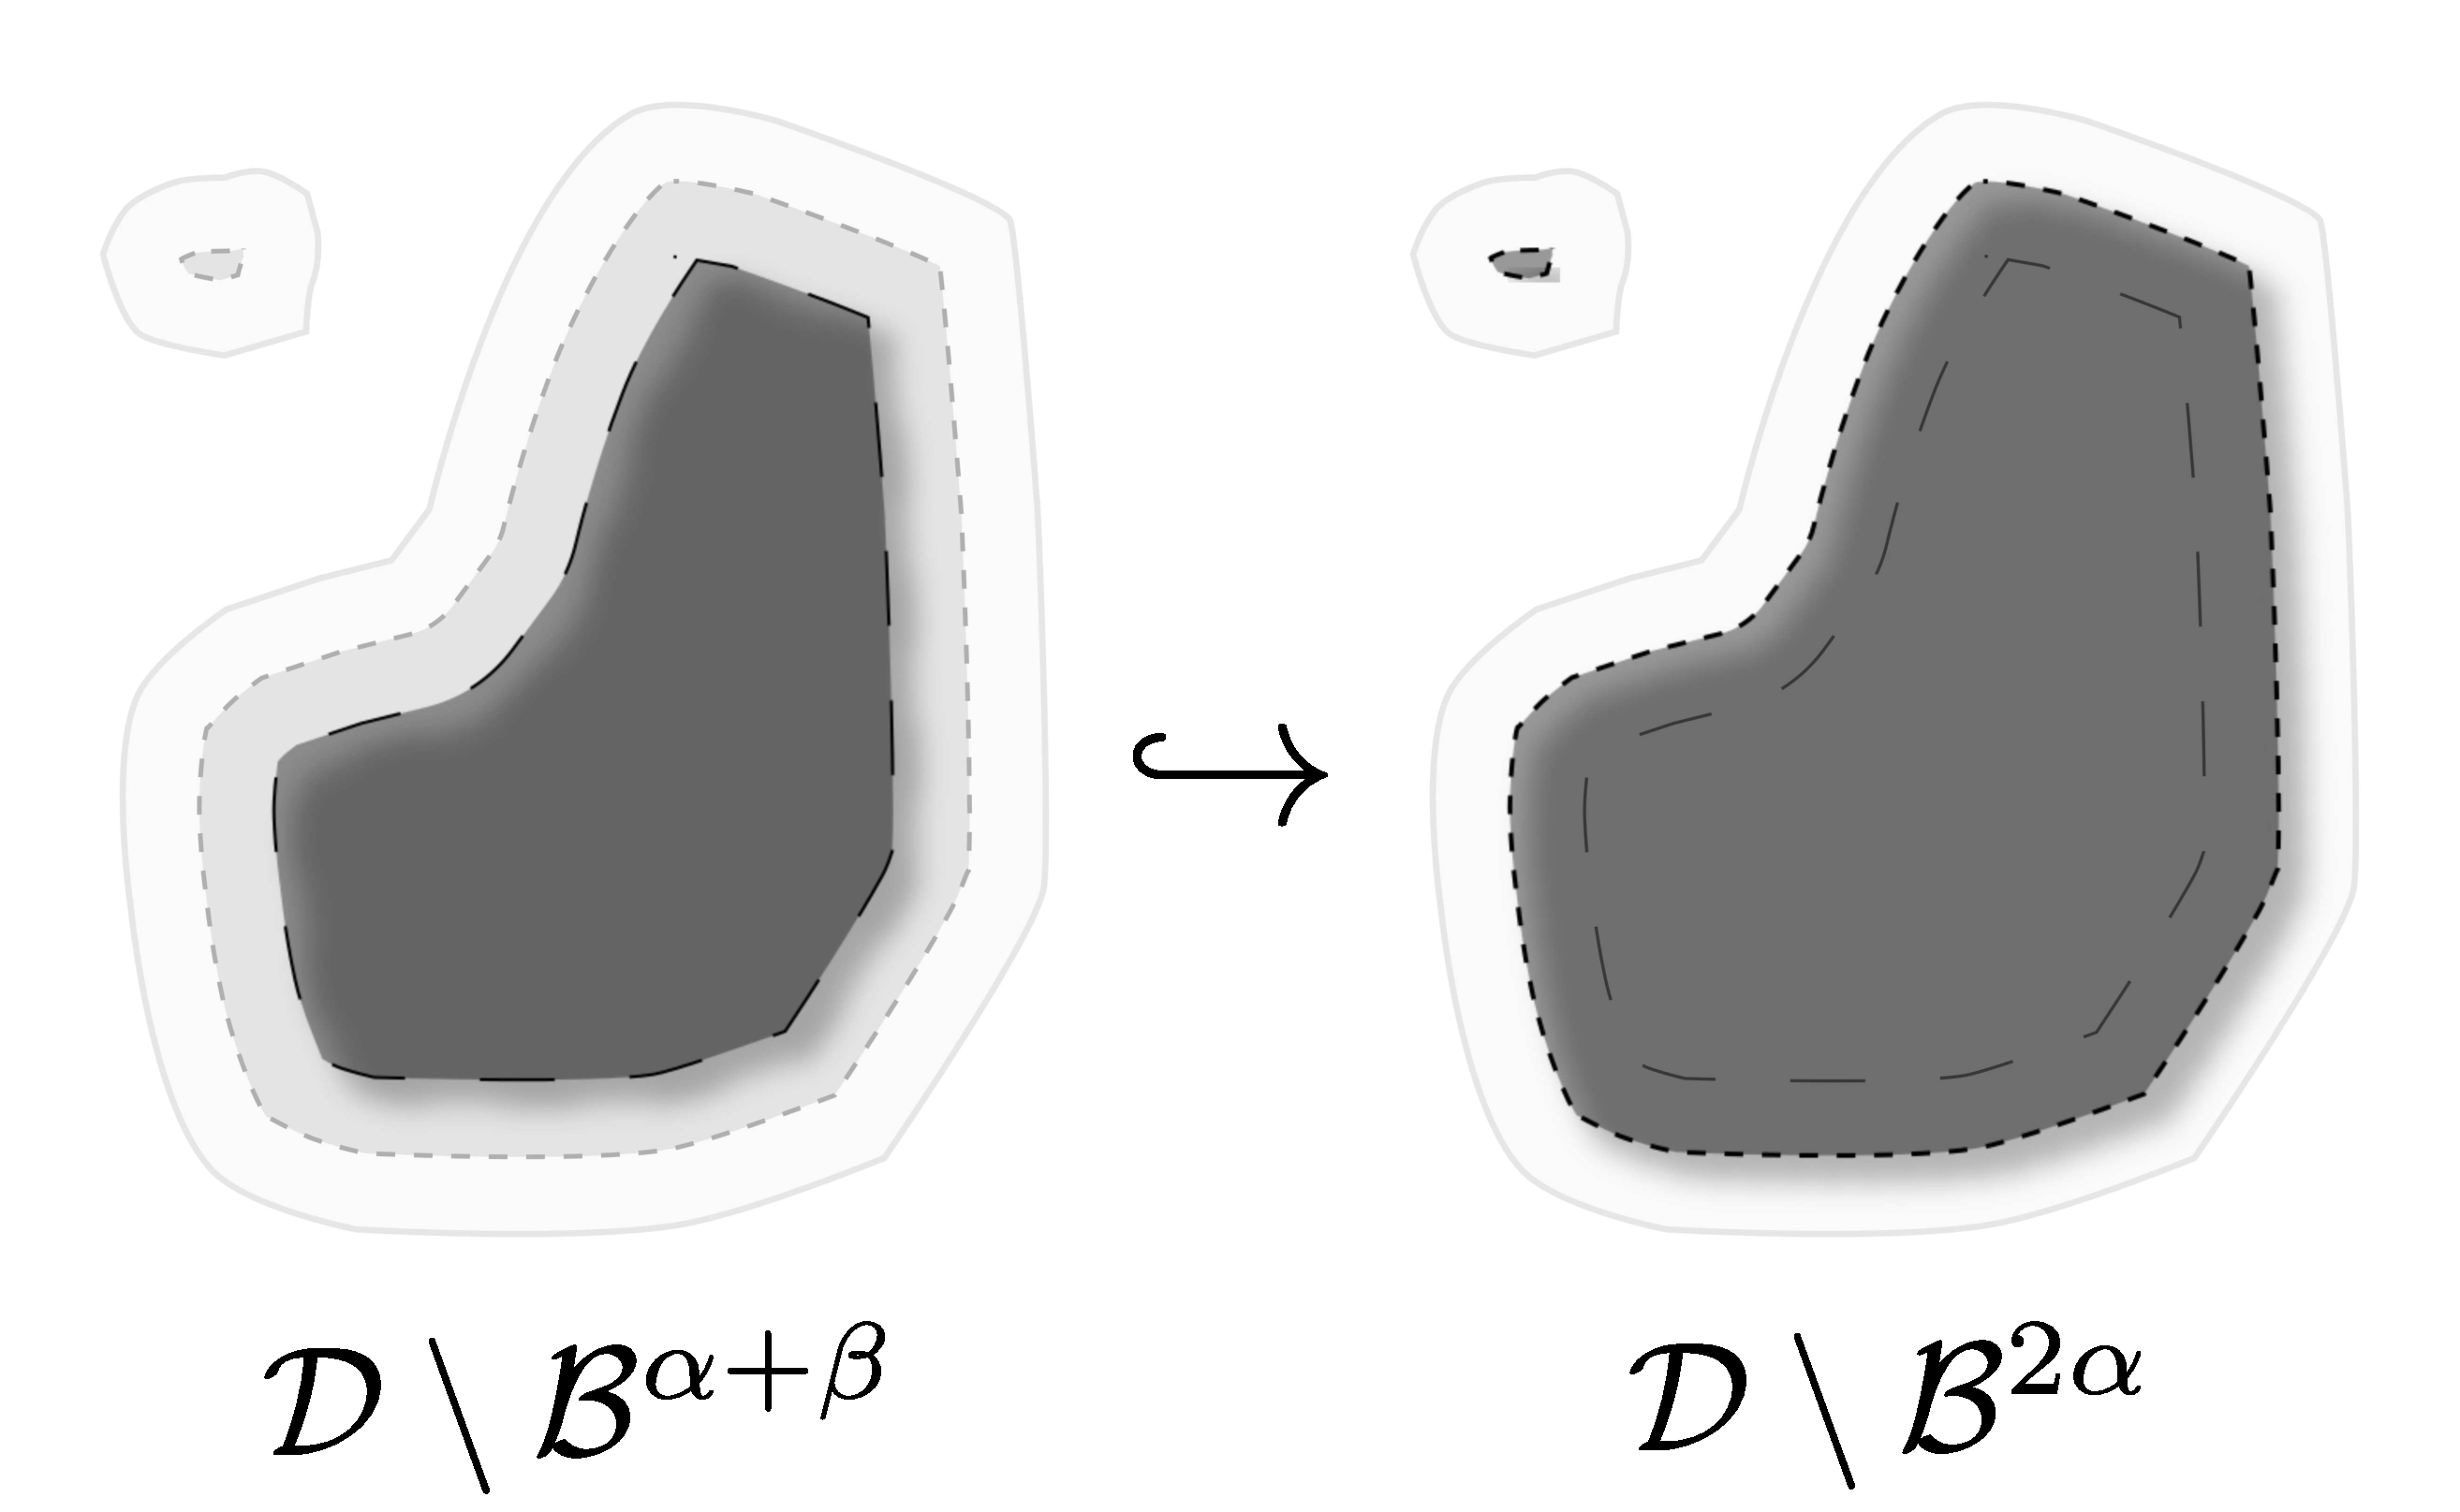
\includegraphics[scale=0.15]{figures/a1_composite.eps}
    \caption{A domain that violates Assumption $1$ as the upper-left component appears in the inclusion from $\D\setminus\B^{\alpha+\beta}$ to $\D\setminus\B^{2\alpha}$.}
    \label{fig:assumption1}
\end{wrapfigure}

Assumption~1 disallows domains with components that are too small to be included in the map from $\D\setminus\B^{\alpha+\beta}\hookrightarrow\D\setminus\B^{2\alpha}$ so we can reliably compare the coverage region to the sampled subset of the domain in terms of the $0$-dimensional homology, or connected components.
Fig.~\ref{fig:assumption1} illustrates a domain in which the induced map is not surjective.

Assumption $2$ requires that the components of $\D\setminus\B^{2\alpha}$ are spaced out well enough so that no components are joined with inclusion into $\D^{2\alpha}$.
This includes regions of a connected component of $\D$ that are ``pinched'' into two in $\D\setminus\B^{2\alpha}$ as well as pairs of components in $\D$ that are too close.
Both are illustrated in Fig.~\ref{fig:assumption2}.
% Fig.~\ref{fig:assumption2} illustrates domains which violate Assumption $2$.

% \vspace{2ex}
\begin{figure}[htbp]
    \centering
    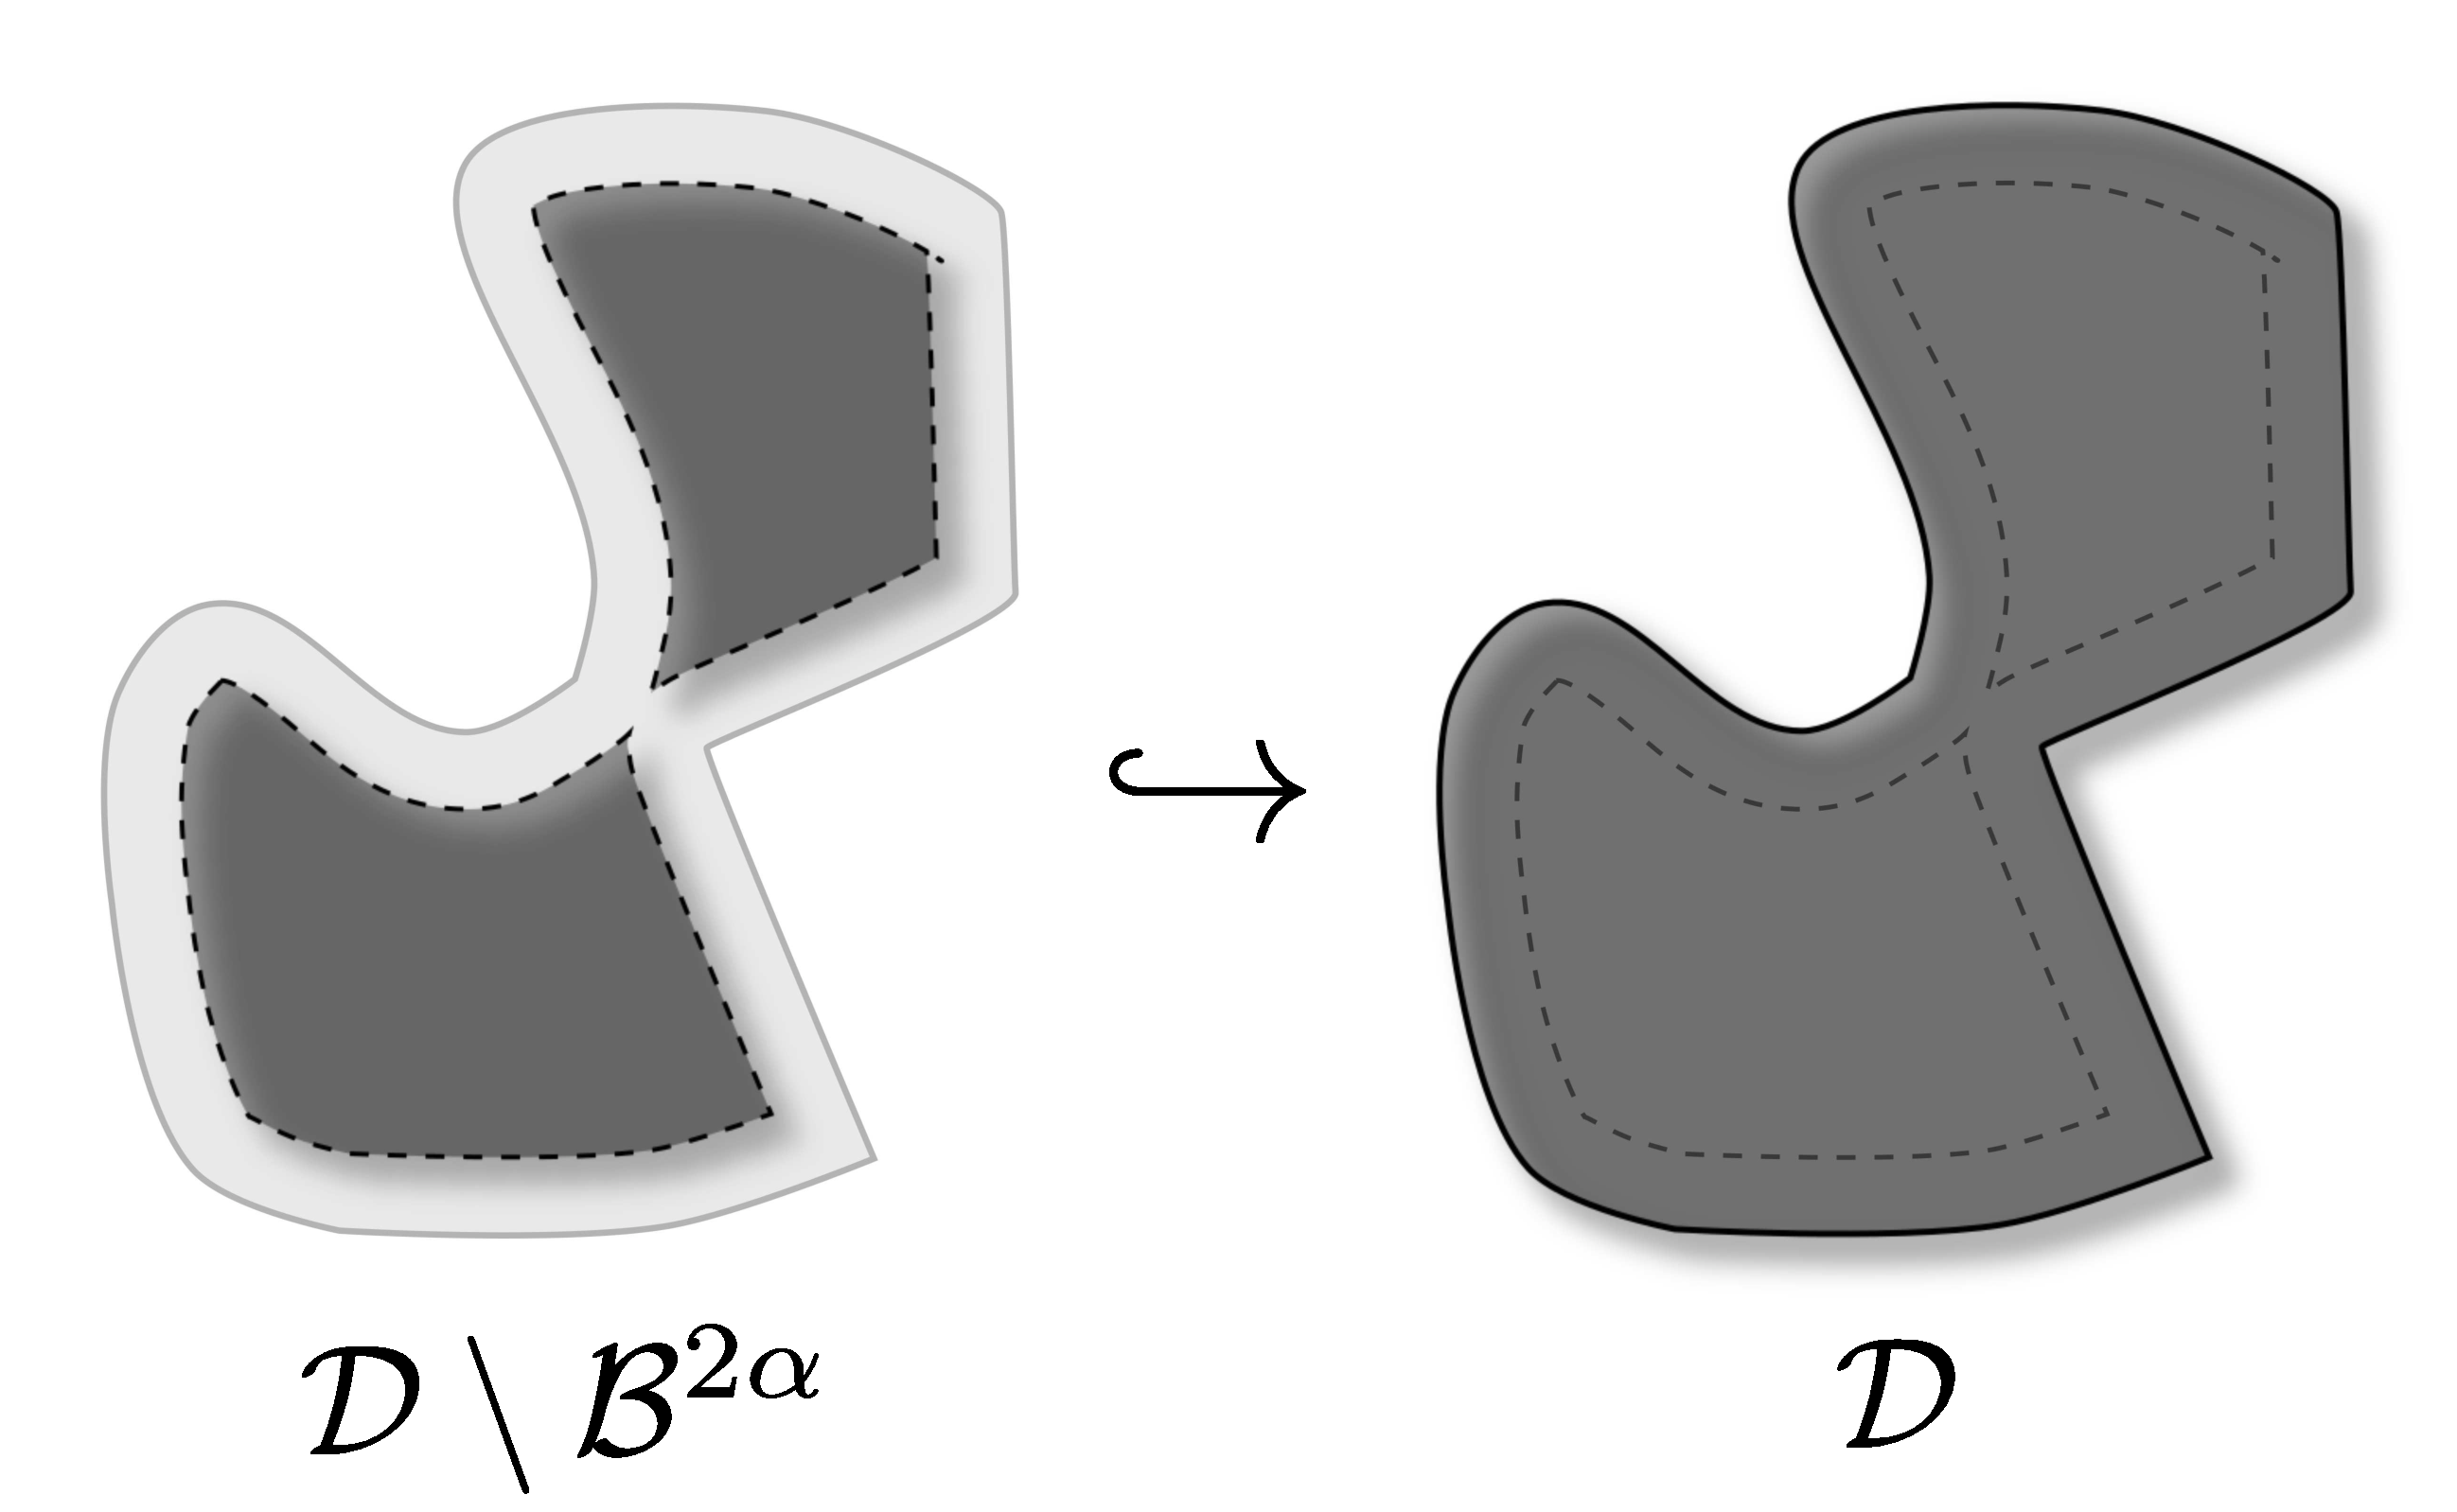
\includegraphics[scale=0.14]{figures/a2_2_composite.eps}\hspace{5ex}
    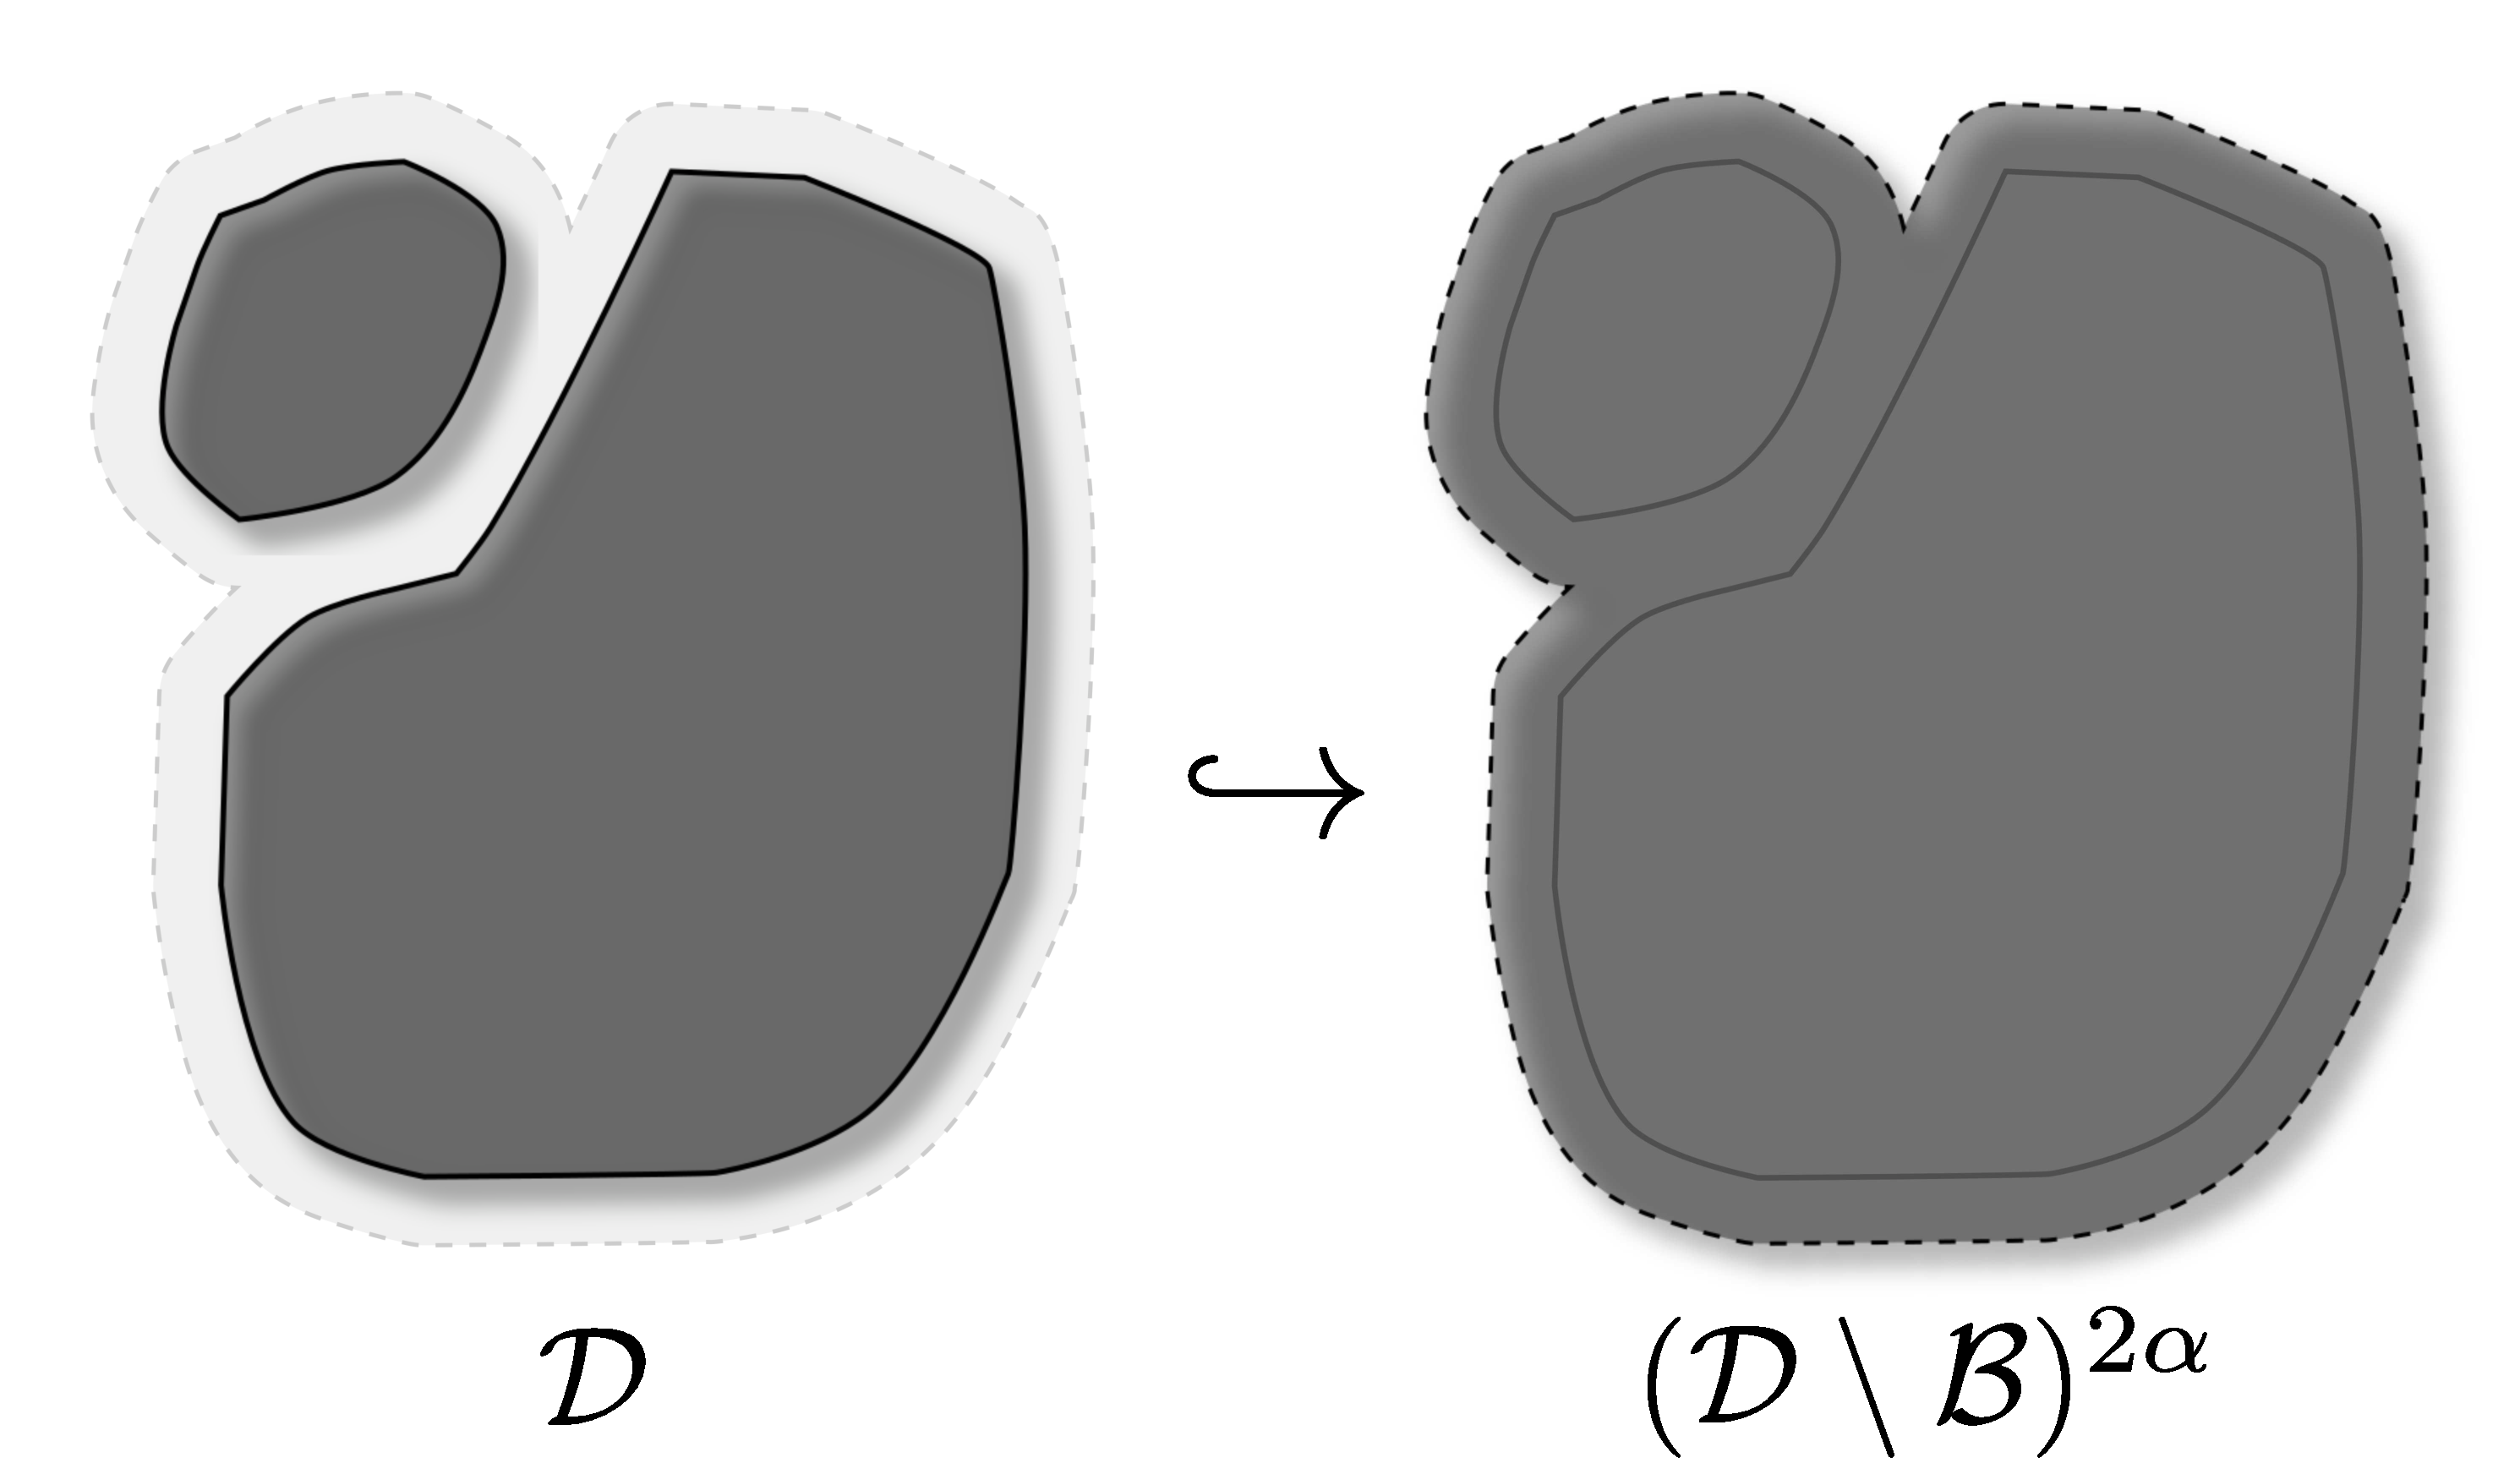
\includegraphics[scale=0.14]{figures/a2_1_composite.eps}
    \caption{Domains which violate Assumption 2 in which components are lost in the inclusions $\D\setminus\B^{2\alpha}\hookrightarrow \D$ and $\D\hookrightarrow (\D\setminus \B)^{2\alpha}$ respectively. In the first case a single component is pinched apart in $\D\setminus\B^{2\alpha}$. In the second, two components which are too close are merged in $(\D\setminus \B)^{2\alpha}$.}
    \label{fig:assumption2}
\end{figure}

Assumptions 0-2 are necessary in order to prove the Geometric TCC (see~\cite{cavanna17when}) and, in particular, Assumption $2$ is necessary for the Algorithmic TCC (Theorem~\ref{thm:algorithmic_tcc}) in order to bound the number of connected components of the shrunken domain $\D\setminus\B^{2\alpha}$.

\subsubsection{Algorithmic TCC}

Given a graph $G = (V, E)$ a \textbf{clique} is a collection of vertices $\sigma\subseteq V$ such that $\{u,v\}\in E$ for all $u,v\in\sigma$.
\begin{definition}
    The \textbf{clique complex} of $G$ is defined to be a simplicial complex with simplices for each clique in $G$.
    \[ \clique(G) := \{ \sigma\subseteq V\mid \forall u,v\in\sigma, \{u,v\}\in E \}. \]

    Given a pair of graphs $(G, H)$ where $H$ is a subgraph of $G$, we will denote the pair of Clique complexes as $\clique(G,H) = (\clique(G),\clique(H))$.
\end{definition}

Let $(\D,\B)$ be a pair of spaces satisfying Assumptions $0$--$2$ for constants $\alpha > 0$, $\beta\geq 3\alpha$.
The input to Algorithm~\ref{alg:rips_certify_coverage} will be a pair of graphs $(G_1, G_2)$, a finite weighted point sample $P\subset \D$ and a subsample $Q=\{p\in P\mid \ball_\alpha(p)\cap\B \neq \emptyset\}$.

\vspace{2ex}
\begin{center}
\setlength{\fboxsep}{2ex}
\fbox{\parbox{0.75\textwidth}{
% \vspace{1ex}\hspace{1ex}
\textbf{Input Assumptions}
    \begin{enumerate}
    \setcounter{enumi}{+2}
        \item The graphs $G_1, G_2$ have a vertex set $P\subset\D$ and subgraphs $G_1[Q], G_2[Q]$ induced by restriction to the vertex set
        \[Q = \{ p\in P\mid \ball_\alpha(p)\cap \B\neq\emptyset \}.\]
        \noeuclidean{\item $\U = \{\ball_\e(p)\mid p\in P\}$ is a good cover for $\e\in\{\alpha,\beta\}$.}
        \kcoverage{\item $\clique_k(G_1)\subseteq\cech_k^\alpha(P)\subseteq\cech_k^\beta(P)\subseteq\clique_k(G_2)$.}
        \nokcoverage{\item $\clique(G_1)\subseteq\cech^\alpha(P)\subseteq\cech^\beta(P)\subseteq\clique(G_2)$.}
        \item Each component of $\D\setminus\B^{2\alpha}$ contains a point in $P$.
        \noeuclidean{\kcoverage{\item There exists a triangulation $\K$ of $\R^d\cup\{\infty\}$ and triangulations of $P_k^\e$ and $Q_k^\e$, $L_\e$ and $M_\e$ respectively, where $M_\e\subset L_\e$ in $\K$, for $\e\in\{\alpha,\beta\}$.}
        \nokcoverage{\item There exists a triangulation $\K$ of $\R^d\cup\{\infty\}$ and triangulations of $P^\e$ and $Q^\e$, $L_\e$ and $M_\e$ respectively, where $M_\e\subset L_\e$ in $\K$, for $\e\in\{\alpha,\beta\}$.}}
    \end{enumerate}
}}\end{center}\vspace{3ex}

The input graphs will be used to construct clique complexes, which by Assumption $5$ can be interleaved with \v Cech complexes at scale $\alpha$ and $\beta$.
% \euclidean{The input graphs will be used to construct Rips complexes which can be interleaved with \v Cech complexes by equation~\ref{eq:jung_inclusion}.}
\noeuclidean{Assumption $4$ allows us to apply the Persistent Nerve Lemma~\cite{chazal08towards}.
Note that Assumption $5$ is satisfied when every clique $\sigma\subseteq G_1$ satisfies $\bigcap_{v\in\sigma} \ball_\alpha(v)\neq \emptyset$ and $\ball_\beta(u)\cap\ball_\beta(v)\neq\emptyset$ implies $\{u,v\}\in E(G_2)$ for all $u, v\in\sigma$.
When the domain $\D$ is equipped with the Euclidean metric, Assumption $5$ is equivalent to the interleaving provided by Jung's theorem (Equation~\ref{eq:jung_inclusion}) where the \kcoverage{$k$-clique complex of $G_1$ can be taken as the $k$-Rips}\nokcoverage{clique complex of $G_1$ can be taken as the Rips} complex of $P$ at scale $\alpha/\jungd$.}
\euclidean{Note that because we have assumed our domain $\D$ is equipped with the Euclidean metric Assumption $4$ is equivalent to the interleaving provided by Jung's theorem (Equation~\ref{eq:jung_inclusion}) where the \kcoverage{$k$-clique complex of $G_1$ can be taken as the $k$-Rips}\nokcoverage{clique complex of $G_1$ can be taken as the Rips} complex of $P$ at scale $\alpha/\jungd$.}
\noeuclidean{Finally, }Assumption \noeuclidean{6}\euclidean{5} is required to prove a bound on the number of connected components of $\D\setminus\B^{2\alpha}$ using a computable combinatorial structure.

% \begin{theorem}[Geometric TCC]\label{thm:geometric_tcc}
%   Given a compact, locally contractible domain $\D\subset\R^d$ with boundary $\B\subset\D$, a sample $P\subset\D$, $Q = \B^\alpha\cap P$ and $i_*:\hom_0(\comp{Q^{\beta}},\comp{P^{\beta}})\to\hom_0(\comp{Q^{\alpha}},\comp{P^{\alpha}})$ where $0\leq\alpha\leq\beta$, if $j_*: \hom_0(\comp{\B^{\alpha+\beta}},\comp{\D^{\alpha+\beta}})\to \hom_0(\comp{\B^{2\alpha}},\comp{\D^{2\alpha}})$ is surjective and $\rank~i_* \ge \rank~j_*$ then $\D_{2\alpha}\subseteq P^\alpha$.
% \end{theorem}

\begin{theorem}[Algorithmic TCC]\label{thm:algorithmic_tcc}
    Consider a pair $(\D,\B)$, a finite point sample $P\subset\D$, and constants $\kcoverage{k,}\alpha,\beta$, where $0 < 3\alpha\leq \beta$, satisfying Assumptions $0$--$\euclidean{5}\noeuclidean{7}$.

    If
    \kcoverage{\[\rank~\hom_d(\clique_k(G_1, G_1[Q])\hookrightarrow \clique_k(G_2, G_2[Q])) =|\textrm{Components}(G_1[P\setminus Q])|\]}
    \nokcoverage{\[\rank~\hom_d(\clique(G_1, G_1[Q])\hookrightarrow \clique(G_2, G_2[Q])) =|\textrm{Components}(G_1[P\setminus Q])|\]}
    then $\D\setminus\B^{2\alpha}\subseteq \kcoverage{P_k^\alpha}\nokcoverage{P^\alpha}$.
\end{theorem}

\subsection{Implementation}

We have included an implementation of the TCC which implements Algorithm~\ref{alg:rips_certify_coverage} for exploratory purposes.

\begin{center}
\begin{minipage}{0.6\textwidth}
    \begin{algorithm}[H]
    	\caption{Check if $\D\setminus B^{2\alpha}\subseteq \kcoverage{P_k^\alpha}\nokcoverage{P^\alpha}$}
    	\label{alg:rips_certify_coverage}
    	\begin{algorithmic}[1]
    		\kcoverage{\Procedure{k-Coverage}{$G_1, G_2, P, Q, k$}}
            \nokcoverage{\Procedure{Coverage}{$G_1, G_2, P, Q$}}
    			\State let $c := |Components(G_1[P\setminus Q])|$
    			\kcoverage{\State let $r := \rank~\hom_d(\clique_k(G_1, G_1[Q])\hookrightarrow \clique_k(G_2, G_2[Q]))$}
    			\nokcoverage{\State let $r := \rank~\hom_d(\clique(G_1, G_1[Q])\hookrightarrow \clique(G_2, G_2[Q]))$}
    			\If{$c=r$}
            \Return True
            \Else ~
            \Return False
    			\EndIf
    		\EndProcedure
    	\end{algorithmic}
    \end{algorithm}
\end{minipage}
\end{center}

A domain $\D\subset\R^2$ is generated by a gaussian random field as a function on the plane by identifying a sublevel set and the surrounding region $\B$ that satisfies our geometric assumptions.

\begin{figure}[htbp]
\centering
    % 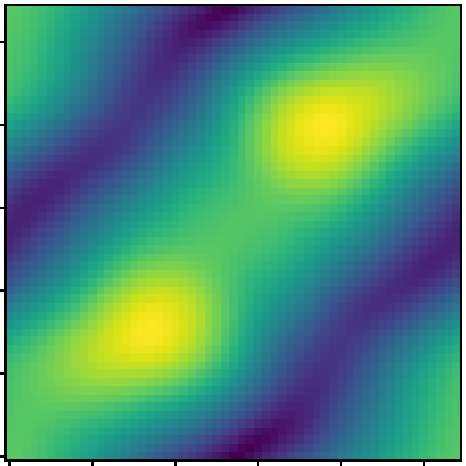
\includegraphics[scale=0.85]{figures/hsn_field.pdf}\hspace{0.5in}
    % 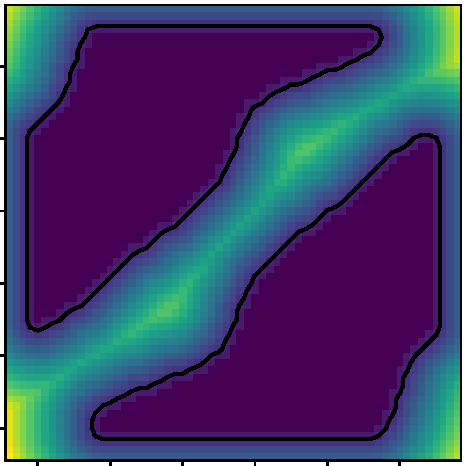
\includegraphics[scale=0.8]{figures/hsn_boundary.pdf}
    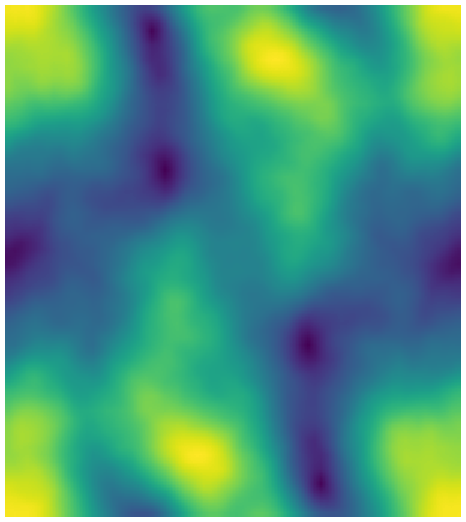
\includegraphics[scale=0.8]{figures/hsn_domain_0.pdf}\hspace{0.5in}
    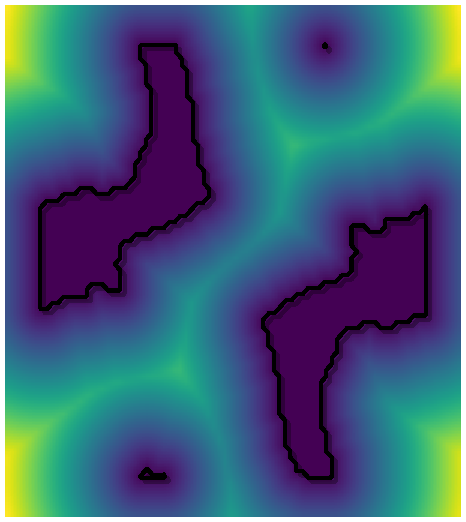
\includegraphics[scale=0.8]{figures/hsn_domain_1.pdf}
    \caption{(Left) A gaussian random field as a function on the plane.
            (Right) The distance to a sublevel set of the function identified as our domain $\D$ with boundary $\B$ in black.}
    \label{fig:hsn}
\end{figure}

We then sample the domain with a collection of points $P\subset\D$ and select a subset $Q$ of $P$ within a fixed distance $\alpha$ of $\B$.
The Dionysus C++ library~\cite{dionysus2} is used to construct the 3-dimensional rips complex of $P$ at scale $\beta = 3\alpha$ in addition to the persistent relative homology of the pair $(\rips^\beta(P), \rips^\beta(Q))$.
The rank of the inclusion \[H_2(\rips^\alpha(P), \rips^\alpha(Q))\to H_2(\rips^\beta(P), \rips^\beta(Q))\] is identified as the number of features in $\dgm_2(\rips^\beta(P), \rips^\beta(P))$ which have not died at scale $\beta$, but were born at scale at most $\alpha$.
This is then compared to the number of connected components in $\rips^\alpha(P\setminus Q)$ as the number of features in $\dgm_0(\rips^\alpha(P\setminus Q))$ that have not died at scale $\alpha$.

\begin{figure}[htbp]
\centering
    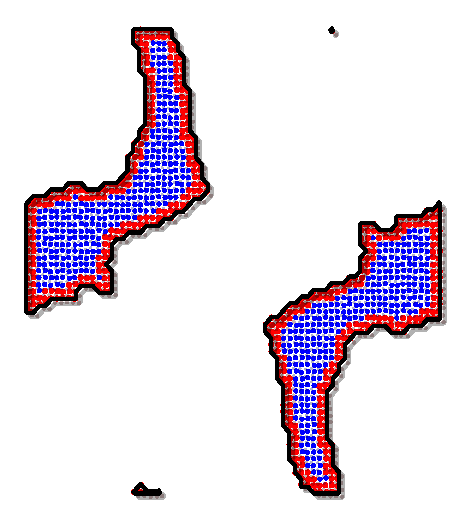
\includegraphics[scale=1.]{figures/hsn_domain_2.pdf}
    \caption{The resulting sampled domain $P$ with $Q$ in red.}
    \label{fig:hsn_domain}
\end{figure}

\begin{figure}[htbp]
\centering
    % 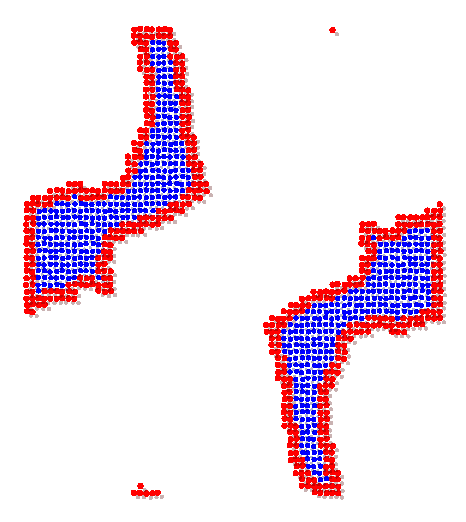
\includegraphics[scale=0.8]{figures/hsn_size_0.pdf}
    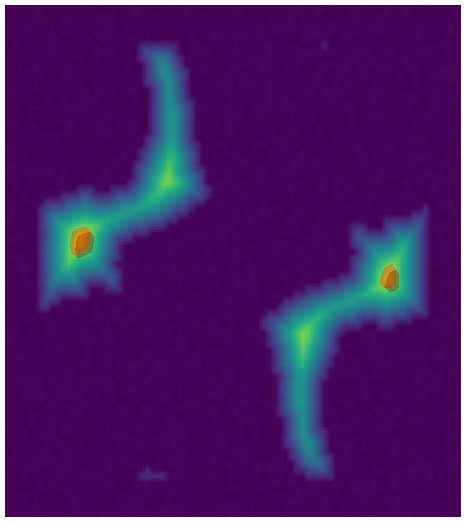
\includegraphics[scale=0.8]{figures/hsn_size_1.pdf}\hspace{0.5in}
    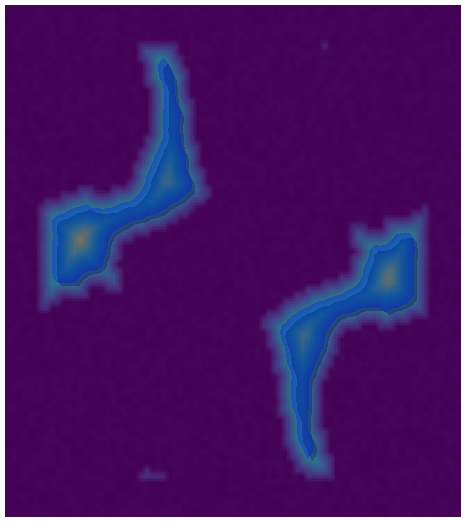
\includegraphics[scale=0.8]{figures/hsn_size_2.pdf}
    \caption{Verification of assumption 1 via sublevel sets of the distance to the complement of $\D$:
            $\D\setminus\B^{\alpha+\beta}$ (left) $\D\setminus\B^{2\alpha}$ (right).}
    \label{fig:hsn_size}
\end{figure}

\begin{figure}[htbp]
\centering
    % 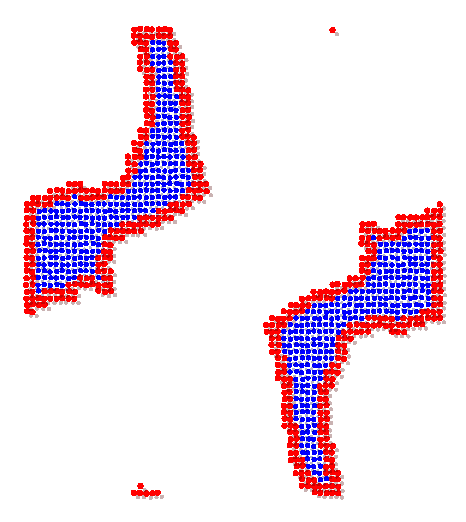
\includegraphics[scale=0.6]{figures/hsn_close_0.pdf}
    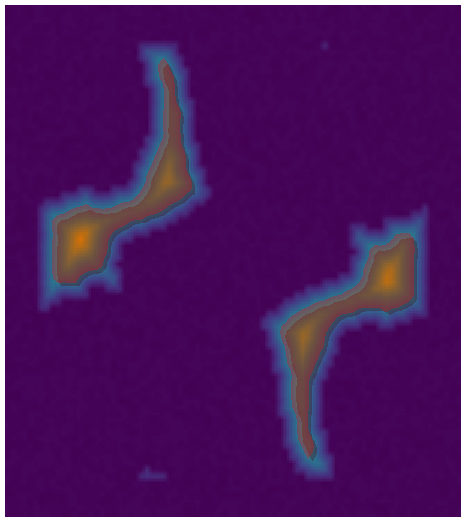
\includegraphics[scale=0.8]{figures/hsn_close_1.pdf}\hspace{0.5in}
    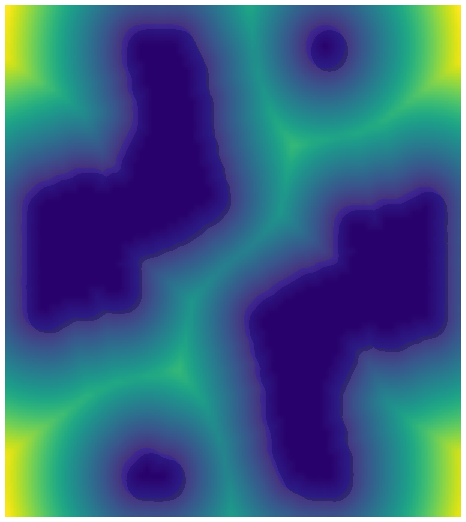
\includegraphics[scale=0.8]{figures/hsn_close_2.pdf}
    \caption{Verification of assumption 2 via sublevel sets of the distance to the complement of $\D$ (left) and the distance to $\D\setminus\B$ (right);
            $\D\setminus\B^{2\alpha}$ (left) $(\D\setminus\B)^{2\alpha}$ (right).}
    \label{fig:hsn_close}
\end{figure}

\begin{figure}[htbp]
\centering
    % 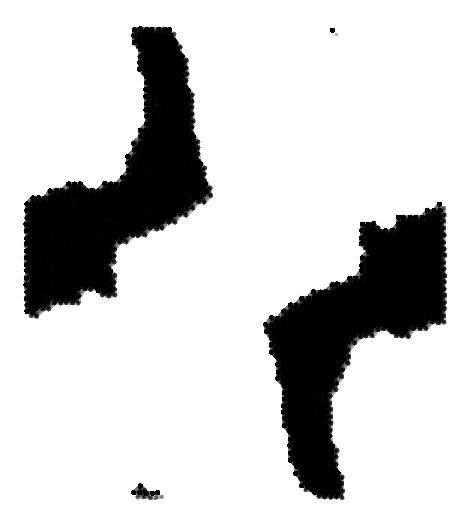
\includegraphics[scale=0.8]{figures/hsn_net_0.pdf}
    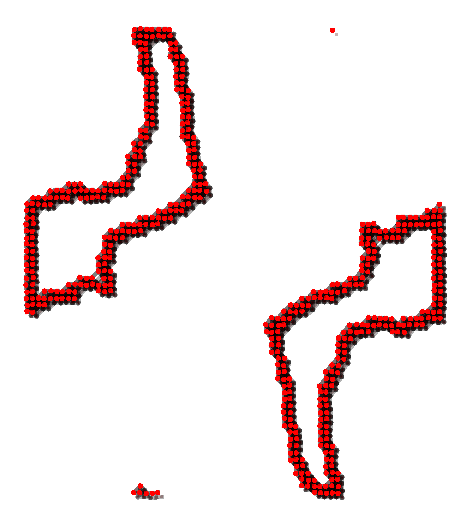
\includegraphics[scale=0.8]{figures/hsn_net_1.pdf}\hspace{0.4in}
    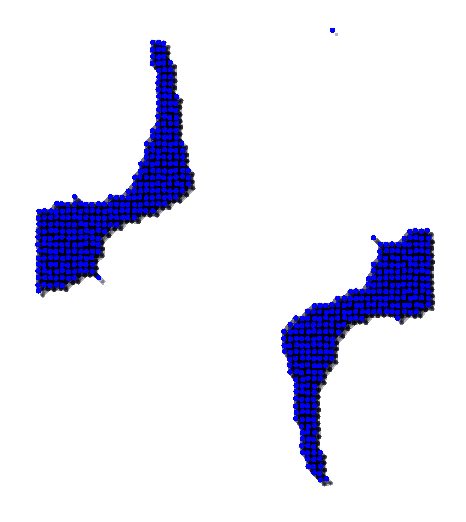
\includegraphics[scale=0.8]{figures/hsn_net_2.pdf}
    \caption{Subcomplexes of $\rips^\alpha(P)$ restricted to $Q$ (left) and $P\setminus Q$ (right).}
    \label{fig:hsn_net}
\end{figure}

% section tcc (end)

% !TeX root = ../main.tex
\section{Conclusion} % (fold)
\label{sec:conclusion}

% section conclusion (end)


\bibliographystyle{plain}
\bibliography{etc/bibliography}
\clearpage

\end{document}
